\documentclass[twoside]{book}

% Packages required by doxygen
\usepackage{fixltx2e}
\usepackage{calc}
\usepackage{doxygen}
\usepackage[export]{adjustbox} % also loads graphicx
\usepackage{graphicx}
\usepackage[utf8]{inputenc}
\usepackage{makeidx}
\usepackage{multicol}
\usepackage{multirow}
\PassOptionsToPackage{warn}{textcomp}
\usepackage{textcomp}
\usepackage[nointegrals]{wasysym}
\usepackage[table]{xcolor}

% Font selection
\usepackage[T1]{fontenc}
\usepackage[scaled=.90]{helvet}
\usepackage{courier}
\usepackage{amssymb}
\usepackage{sectsty}
\renewcommand{\familydefault}{\sfdefault}
\allsectionsfont{%
  \fontseries{bc}\selectfont%
  \color{darkgray}%
}
\renewcommand{\DoxyLabelFont}{%
  \fontseries{bc}\selectfont%
  \color{darkgray}%
}
\newcommand{\+}{\discretionary{\mbox{\scriptsize$\hookleftarrow$}}{}{}}

% Page & text layout
\usepackage{geometry}
\geometry{%
  a4paper,%
  top=2.5cm,%
  bottom=2.5cm,%
  left=2.5cm,%
  right=2.5cm%
}
\tolerance=750
\hfuzz=15pt
\hbadness=750
\setlength{\emergencystretch}{15pt}
\setlength{\parindent}{0cm}
\setlength{\parskip}{3ex plus 2ex minus 2ex}
\makeatletter
\renewcommand{\paragraph}{%
  \@startsection{paragraph}{4}{0ex}{-1.0ex}{1.0ex}{%
    \normalfont\normalsize\bfseries\SS@parafont%
  }%
}
\renewcommand{\subparagraph}{%
  \@startsection{subparagraph}{5}{0ex}{-1.0ex}{1.0ex}{%
    \normalfont\normalsize\bfseries\SS@subparafont%
  }%
}
\makeatother

% Headers & footers
\usepackage{fancyhdr}
\pagestyle{fancyplain}
\fancyhead[LE]{\fancyplain{}{\bfseries\thepage}}
\fancyhead[CE]{\fancyplain{}{}}
\fancyhead[RE]{\fancyplain{}{\bfseries\leftmark}}
\fancyhead[LO]{\fancyplain{}{\bfseries\rightmark}}
\fancyhead[CO]{\fancyplain{}{}}
\fancyhead[RO]{\fancyplain{}{\bfseries\thepage}}
\fancyfoot[LE]{\fancyplain{}{}}
\fancyfoot[CE]{\fancyplain{}{}}
\fancyfoot[RE]{\fancyplain{}{\bfseries\scriptsize Generated by Doxygen }}
\fancyfoot[LO]{\fancyplain{}{\bfseries\scriptsize Generated by Doxygen }}
\fancyfoot[CO]{\fancyplain{}{}}
\fancyfoot[RO]{\fancyplain{}{}}
\renewcommand{\footrulewidth}{0.4pt}
\renewcommand{\chaptermark}[1]{%
  \markboth{#1}{}%
}
\renewcommand{\sectionmark}[1]{%
  \markright{\thesection\ #1}%
}

% Indices & bibliography
\usepackage{natbib}
\usepackage[titles]{tocloft}
\setcounter{tocdepth}{3}
\setcounter{secnumdepth}{5}
\makeindex

% Hyperlinks (required, but should be loaded last)
\usepackage{ifpdf}
\ifpdf
  \usepackage[pdftex,pagebackref=true]{hyperref}
\else
  \usepackage[ps2pdf,pagebackref=true]{hyperref}
\fi
\hypersetup{%
  colorlinks=true,%
  linkcolor=blue,%
  citecolor=blue,%
  unicode%
}

% Custom commands
\newcommand{\clearemptydoublepage}{%
  \newpage{\pagestyle{empty}\cleardoublepage}%
}

\usepackage{caption}
\captionsetup{labelsep=space,justification=centering,font={bf},singlelinecheck=off,skip=4pt,position=top}

%===== C O N T E N T S =====

\begin{document}

% Titlepage & ToC
\hypersetup{pageanchor=false,
             bookmarksnumbered=true,
             pdfencoding=unicode
            }
\pagenumbering{alph}
\begin{titlepage}
\vspace*{7cm}
\begin{center}%
{\Large M\+PE }\\
\vspace*{1cm}
{\large Generated by Doxygen 1.8.13}\\
\end{center}
\end{titlepage}
\clearemptydoublepage
\pagenumbering{roman}
\tableofcontents
\clearemptydoublepage
\pagenumbering{arabic}
\hypersetup{pageanchor=true}

%--- Begin generated contents ---
\chapter{M\+PE}
\label{md__c_1__users__walter__source__repos__m_p_e__r_e_a_d_m_e}
\Hypertarget{md__c_1__users__walter__source__repos__m_p_e__r_e_a_d_m_e}
Message Passing Engine 
\chapter{Namespace Index}
\section{Namespace List}
Here is a list of all namespaces with brief descriptions\+:\begin{DoxyCompactList}
\item\contentsline{section}{\hyperlink{namespace_m_p_e}{M\+PE} }{\pageref{namespace_m_p_e}}{}
\item\contentsline{section}{\hyperlink{namespace_m_p_e_1_1_tag}{M\+P\+E\+::\+Tag} }{\pageref{namespace_m_p_e_1_1_tag}}{}
\item\contentsline{section}{\hyperlink{namespace_m_p_e_1_1_tag_1_1_data_manager}{M\+P\+E\+::\+Tag\+::\+Data\+Manager} }{\pageref{namespace_m_p_e_1_1_tag_1_1_data_manager}}{}
\end{DoxyCompactList}

\chapter{Hierarchical Index}
\section{Class Hierarchy}
This inheritance list is sorted roughly, but not completely, alphabetically\+:\begin{DoxyCompactList}
\item \contentsline{section}{M\+PE\+:\+:Base\+Manager\+Entity\+Entry\+Block}{\pageref{struct_m_p_e_1_1_base_manager_entity_entry_block}}{}
\begin{DoxyCompactList}
\item \contentsline{section}{M\+PE\+:\+:Data\+Manager\+:\+:Entity\+Data}{\pageref{struct_m_p_e_1_1_data_manager_1_1_entity_data}}{}
\end{DoxyCompactList}
\item \contentsline{section}{M\+PE\+:\+:Data\+Manager\+:\+:Data}{\pageref{struct_m_p_e_1_1_data_manager_1_1_data}}{}
\item \contentsline{section}{Profiler\+:\+:Data}{\pageref{struct_profiler_1_1_data}}{}
\item \contentsline{section}{M\+PE\+:\+:Data\+Manager\+:\+:Data\+Buffer}{\pageref{struct_m_p_e_1_1_data_manager_1_1_data_buffer}}{}
\item \contentsline{section}{M\+PE\+:\+:Entity}{\pageref{struct_m_p_e_1_1_entity}}{}
\item \contentsline{section}{M\+PE\+:\+:Entity\+Hasher}{\pageref{struct_m_p_e_1_1_entity_hasher}}{}
\item \contentsline{section}{M\+PE\+:\+:Data\+Manager\+:\+:Entry\+Header}{\pageref{struct_m_p_e_1_1_data_manager_1_1_entry_header}}{}
\item \contentsline{section}{M\+PE\+:\+:Msg}{\pageref{struct_m_p_e_1_1_msg}}{}
\item \contentsline{section}{M\+PE\+:\+:Msg\+Comp}{\pageref{struct_m_p_e_1_1_msg_comp}}{}
\item \contentsline{section}{Profiler}{\pageref{class_profiler}}{}
\item \contentsline{section}{M\+PE\+:\+:Thread}{\pageref{class_m_p_e_1_1_thread}}{}
\begin{DoxyCompactList}
\item \contentsline{section}{M\+PE\+:\+:Manager}{\pageref{class_m_p_e_1_1_manager}}{}
\begin{DoxyCompactList}
\item \contentsline{section}{M\+PE\+:\+:Data\+Manager}{\pageref{class_m_p_e_1_1_data_manager}}{}
\end{DoxyCompactList}
\end{DoxyCompactList}
\item \contentsline{section}{M\+PE\+:\+:Thread\+Message\+Controller}{\pageref{class_m_p_e_1_1_thread_message_controller}}{}
\item \contentsline{section}{M\+PE\+:\+:Data\+Manager\+:\+:Value}{\pageref{struct_m_p_e_1_1_data_manager_1_1_value}}{}
\item \contentsline{section}{M\+PE\+:\+:Data\+Manager\+:\+:Value\+\_\+\+Buffer}{\pageref{struct_m_p_e_1_1_data_manager_1_1_value___buffer}}{}
\end{DoxyCompactList}

\chapter{Class Index}
\section{Class List}
Here are the classes, structs, unions and interfaces with brief descriptions\+:\begin{DoxyCompactList}
\item\contentsline{section}{\hyperlink{struct_tag}{Tag} }{\pageref{struct_tag}}{}
\item\contentsline{section}{\hyperlink{class_m_p_e_1_1_thread}{M\+P\+E\+::\+Thread} \\*The thread base class }{\pageref{class_m_p_e_1_1_thread}}{}
\item\contentsline{section}{\hyperlink{class_m_p_e_1_1_thread_message_controller}{M\+P\+E\+::\+Thread\+Message\+Controller} \\*The \hyperlink{class_m_p_e_1_1_thread_message_controller}{Thread\+Message\+Controller} initiates threads and handles the communication between them }{\pageref{class_m_p_e_1_1_thread_message_controller}}{}
\end{DoxyCompactList}

\chapter{File Index}
\section{File List}
Here is a list of all files with brief descriptions\+:\begin{DoxyCompactList}
\item\contentsline{section}{\hyperlink{_data_manager_8cpp}{Data\+Manager.\+cpp} }{\pageref{_data_manager_8cpp}}{}
\item\contentsline{section}{\hyperlink{_data_manager_8h}{Data\+Manager.\+h} }{\pageref{_data_manager_8h}}{}
\item\contentsline{section}{\hyperlink{_data_mangager_messages_8h}{Data\+Mangager\+Messages.\+h} }{\pageref{_data_mangager_messages_8h}}{}
\item\contentsline{section}{\hyperlink{_entity_8cpp}{Entity.\+cpp} }{\pageref{_entity_8cpp}}{}
\item\contentsline{section}{\hyperlink{_entity_8h}{Entity.\+h} }{\pageref{_entity_8h}}{}
\item\contentsline{section}{\hyperlink{_manager_8cpp}{Manager.\+cpp} }{\pageref{_manager_8cpp}}{}
\item\contentsline{section}{\hyperlink{_manager_8h}{Manager.\+h} }{\pageref{_manager_8h}}{}
\item\contentsline{section}{\hyperlink{_m_p_e___tag_8h}{M\+P\+E\+\_\+\+Tag.\+h} }{\pageref{_m_p_e___tag_8h}}{}
\item\contentsline{section}{\hyperlink{_msg_8h}{Msg.\+h} }{\pageref{_msg_8h}}{}
\item\contentsline{section}{\hyperlink{_profiler_8h}{Profiler.\+h} }{\pageref{_profiler_8h}}{}
\item\contentsline{section}{\hyperlink{_source_8cpp}{Source.\+cpp} }{\pageref{_source_8cpp}}{}
\item\contentsline{section}{\hyperlink{_thread_8cpp}{Thread.\+cpp} }{\pageref{_thread_8cpp}}{}
\item\contentsline{section}{\hyperlink{_thread_8h}{Thread.\+h} }{\pageref{_thread_8h}}{}
\item\contentsline{section}{\hyperlink{_thread_message_controller_8cpp}{Thread\+Message\+Controller.\+cpp} }{\pageref{_thread_message_controller_8cpp}}{}
\item\contentsline{section}{\hyperlink{_thread_message_controller_8h}{Thread\+Message\+Controller.\+h} }{\pageref{_thread_message_controller_8h}}{}
\end{DoxyCompactList}

\chapter{Namespace Documentation}
\hypertarget{namespace_m_p_e}{}\section{M\+PE Namespace Reference}
\label{namespace_m_p_e}\index{M\+PE@{M\+PE}}
\subsection*{Namespaces}
\begin{DoxyCompactItemize}
\item 
 \hyperlink{namespace_m_p_e_1_1_tag}{Tag}
\end{DoxyCompactItemize}
\subsection*{Classes}
\begin{DoxyCompactItemize}
\item 
struct \hyperlink{struct_m_p_e_1_1_base_manager_entity_entry_block}{Base\+Manager\+Entity\+Entry\+Block}
\begin{DoxyCompactList}\small\item\em The memory where the data for each entity entry is held. \end{DoxyCompactList}\item 
class \hyperlink{class_m_p_e_1_1_data_manager}{Data\+Manager}
\begin{DoxyCompactList}\small\item\em The \hyperlink{class_m_p_e_1_1_data_manager}{Data\+Manager} is used to associate basic datatypes to an entity. \end{DoxyCompactList}\item 
struct \hyperlink{struct_m_p_e_1_1_entity}{Entity}
\begin{DoxyCompactList}\small\item\em \hyperlink{struct_m_p_e_1_1_entity}{Entity} is essentially an id. \end{DoxyCompactList}\item 
struct \hyperlink{struct_m_p_e_1_1_entity_hasher}{Entity\+Hasher}
\item 
class \hyperlink{class_m_p_e_1_1_manager}{Manager}
\begin{DoxyCompactList}\small\item\em The manager base class. \end{DoxyCompactList}\item 
struct \hyperlink{struct_m_p_e_1_1_msg}{Msg}
\item 
struct \hyperlink{struct_m_p_e_1_1_msg_comp}{Msg\+Comp}
\item 
class \hyperlink{class_m_p_e_1_1_thread}{Thread}
\begin{DoxyCompactList}\small\item\em The thread base class. \end{DoxyCompactList}\item 
class \hyperlink{class_m_p_e_1_1_thread_message_controller}{Thread\+Message\+Controller}
\begin{DoxyCompactList}\small\item\em The \hyperlink{class_m_p_e_1_1_thread_message_controller}{Thread\+Message\+Controller} initiates threads. \end{DoxyCompactList}\end{DoxyCompactItemize}
\subsection*{Typedefs}
\begin{DoxyCompactItemize}
\item 
typedef uint32\+\_\+t \hyperlink{namespace_m_p_e_a16447295e3105bd2ba2a9ea303566175}{thread\+Identifier}
\end{DoxyCompactItemize}
\subsection*{Functions}
\begin{DoxyCompactItemize}
\item 
const void \hyperlink{namespace_m_p_e_a9485a8e81a058e9f485fa13c60c6d1ef}{Thread\+Entry} (\hyperlink{class_m_p_e_1_1_thread}{Thread} $\ast$thread)
\end{DoxyCompactItemize}
\subsection*{Variables}
\begin{DoxyCompactItemize}
\item 
static uint32\+\_\+t \hyperlink{namespace_m_p_e_a6874547713c4758aae159fa87c365d8e}{Src\+\_\+\+Thread\+Message\+Controller} = 0
\item 
static uint32\+\_\+t \hyperlink{namespace_m_p_e_a0a698f47d1ab10c44a414685c36494f1}{Msg\+\_\+\+Any\+\_\+\+Src} = U\+I\+N\+T32\+\_\+\+M\+AX
\end{DoxyCompactItemize}


\subsection{Detailed Description}
The basic tags used during message passing. 

\subsection{Typedef Documentation}
\mbox{\Hypertarget{namespace_m_p_e_a16447295e3105bd2ba2a9ea303566175}\label{namespace_m_p_e_a16447295e3105bd2ba2a9ea303566175}} 
\index{M\+PE@{M\+PE}!thread\+Identifier@{thread\+Identifier}}
\index{thread\+Identifier@{thread\+Identifier}!M\+PE@{M\+PE}}
\subsubsection{\texorpdfstring{thread\+Identifier}{threadIdentifier}}
{\footnotesize\ttfamily typedef uint32\+\_\+t \hyperlink{namespace_m_p_e_a16447295e3105bd2ba2a9ea303566175}{M\+P\+E\+::thread\+Identifier}}



\subsection{Function Documentation}
\mbox{\Hypertarget{namespace_m_p_e_a9485a8e81a058e9f485fa13c60c6d1ef}\label{namespace_m_p_e_a9485a8e81a058e9f485fa13c60c6d1ef}} 
\index{M\+PE@{M\+PE}!Thread\+Entry@{Thread\+Entry}}
\index{Thread\+Entry@{Thread\+Entry}!M\+PE@{M\+PE}}
\subsubsection{\texorpdfstring{Thread\+Entry()}{ThreadEntry()}}
{\footnotesize\ttfamily const void M\+P\+E\+::\+Thread\+Entry (\begin{DoxyParamCaption}\item[{\hyperlink{class_m_p_e_1_1_thread}{Thread} $\ast$}]{thread }\end{DoxyParamCaption})}



\subsection{Variable Documentation}
\mbox{\Hypertarget{namespace_m_p_e_a0a698f47d1ab10c44a414685c36494f1}\label{namespace_m_p_e_a0a698f47d1ab10c44a414685c36494f1}} 
\index{M\+PE@{M\+PE}!Msg\+\_\+\+Any\+\_\+\+Src@{Msg\+\_\+\+Any\+\_\+\+Src}}
\index{Msg\+\_\+\+Any\+\_\+\+Src@{Msg\+\_\+\+Any\+\_\+\+Src}!M\+PE@{M\+PE}}
\subsubsection{\texorpdfstring{Msg\+\_\+\+Any\+\_\+\+Src}{Msg\_Any\_Src}}
{\footnotesize\ttfamily uint32\+\_\+t M\+P\+E\+::\+Msg\+\_\+\+Any\+\_\+\+Src = U\+I\+N\+T32\+\_\+\+M\+AX\hspace{0.3cm}{\ttfamily [static]}}

Specify to allow messages from any source. \mbox{\Hypertarget{namespace_m_p_e_a6874547713c4758aae159fa87c365d8e}\label{namespace_m_p_e_a6874547713c4758aae159fa87c365d8e}} 
\index{M\+PE@{M\+PE}!Src\+\_\+\+Thread\+Message\+Controller@{Src\+\_\+\+Thread\+Message\+Controller}}
\index{Src\+\_\+\+Thread\+Message\+Controller@{Src\+\_\+\+Thread\+Message\+Controller}!M\+PE@{M\+PE}}
\subsubsection{\texorpdfstring{Src\+\_\+\+Thread\+Message\+Controller}{Src\_ThreadMessageController}}
{\footnotesize\ttfamily uint32\+\_\+t M\+P\+E\+::\+Src\+\_\+\+Thread\+Message\+Controller = 0\hspace{0.3cm}{\ttfamily [static]}}

Soruce 0 is reserved for \hyperlink{class_m_p_e_1_1_thread_message_controller}{Thread\+Message\+Controller}. 
\hypertarget{namespace_m_p_e_1_1_tag}{}\section{M\+PE\+:\+:Tag Namespace Reference}
\label{namespace_m_p_e_1_1_tag}\index{M\+P\+E\+::\+Tag@{M\+P\+E\+::\+Tag}}
\subsection*{Namespaces}
\begin{DoxyCompactItemize}
\item 
 \hyperlink{namespace_m_p_e_1_1_tag_1_1_data_manager}{Data\+Manager}
\end{DoxyCompactItemize}
\subsection*{Variables}
\begin{DoxyCompactItemize}
\item 
static const uint32\+\_\+t \hyperlink{namespace_m_p_e_1_1_tag_aa5b0456e2af78c51452dd5a5a9b39b8c}{Any} = 0
\item 
static const uint32\+\_\+t \hyperlink{namespace_m_p_e_1_1_tag_abc1f55c07827fa1883742f19dba494a4}{Shutdown} = 1
\end{DoxyCompactItemize}


\subsection{Variable Documentation}
\mbox{\Hypertarget{namespace_m_p_e_1_1_tag_aa5b0456e2af78c51452dd5a5a9b39b8c}\label{namespace_m_p_e_1_1_tag_aa5b0456e2af78c51452dd5a5a9b39b8c}} 
\index{M\+P\+E\+::\+Tag@{M\+P\+E\+::\+Tag}!Any@{Any}}
\index{Any@{Any}!M\+P\+E\+::\+Tag@{M\+P\+E\+::\+Tag}}
\subsubsection{\texorpdfstring{Any}{Any}}
{\footnotesize\ttfamily const uint32\+\_\+t M\+P\+E\+::\+Tag\+::\+Any = 0\hspace{0.3cm}{\ttfamily [static]}}

\mbox{\Hypertarget{namespace_m_p_e_1_1_tag_abc1f55c07827fa1883742f19dba494a4}\label{namespace_m_p_e_1_1_tag_abc1f55c07827fa1883742f19dba494a4}} 
\index{M\+P\+E\+::\+Tag@{M\+P\+E\+::\+Tag}!Shutdown@{Shutdown}}
\index{Shutdown@{Shutdown}!M\+P\+E\+::\+Tag@{M\+P\+E\+::\+Tag}}
\subsubsection{\texorpdfstring{Shutdown}{Shutdown}}
{\footnotesize\ttfamily const uint32\+\_\+t M\+P\+E\+::\+Tag\+::\+Shutdown = 1\hspace{0.3cm}{\ttfamily [static]}}


\hypertarget{namespace_m_p_e_1_1_tag_1_1_data_manager}{}\section{M\+PE\+:\+:Tag\+:\+:Data\+Manager Namespace Reference}
\label{namespace_m_p_e_1_1_tag_1_1_data_manager}\index{M\+P\+E\+::\+Tag\+::\+Data\+Manager@{M\+P\+E\+::\+Tag\+::\+Data\+Manager}}
\subsection*{Variables}
\begin{DoxyCompactItemize}
\item 
static const uint32\+\_\+t \hyperlink{namespace_m_p_e_1_1_tag_1_1_data_manager_a0752ea1b8c0896c530b94efeed0d76cc}{Register\+Entity} = 2
\end{DoxyCompactItemize}


\subsection{Variable Documentation}
\mbox{\Hypertarget{namespace_m_p_e_1_1_tag_1_1_data_manager_a0752ea1b8c0896c530b94efeed0d76cc}\label{namespace_m_p_e_1_1_tag_1_1_data_manager_a0752ea1b8c0896c530b94efeed0d76cc}} 
\index{M\+P\+E\+::\+Tag\+::\+Data\+Manager@{M\+P\+E\+::\+Tag\+::\+Data\+Manager}!Register\+Entity@{Register\+Entity}}
\index{Register\+Entity@{Register\+Entity}!M\+P\+E\+::\+Tag\+::\+Data\+Manager@{M\+P\+E\+::\+Tag\+::\+Data\+Manager}}
\subsubsection{\texorpdfstring{Register\+Entity}{RegisterEntity}}
{\footnotesize\ttfamily const uint32\+\_\+t M\+P\+E\+::\+Tag\+::\+Data\+Manager\+::\+Register\+Entity = 2\hspace{0.3cm}{\ttfamily [static]}}


\chapter{Class Documentation}
\hypertarget{struct_m_p_e_1_1_base_manager_entity_entry_block}{}\section{M\+PE\+:\+:Base\+Manager\+Entity\+Entry\+Block Struct Reference}
\label{struct_m_p_e_1_1_base_manager_entity_entry_block}\index{M\+P\+E\+::\+Base\+Manager\+Entity\+Entry\+Block@{M\+P\+E\+::\+Base\+Manager\+Entity\+Entry\+Block}}


The memory where the data for each entity entry is held.  




{\ttfamily \#include $<$Manager.\+h$>$}

Inheritance diagram for M\+PE\+:\+:Base\+Manager\+Entity\+Entry\+Block\+:\begin{figure}[H]
\begin{center}
\leavevmode
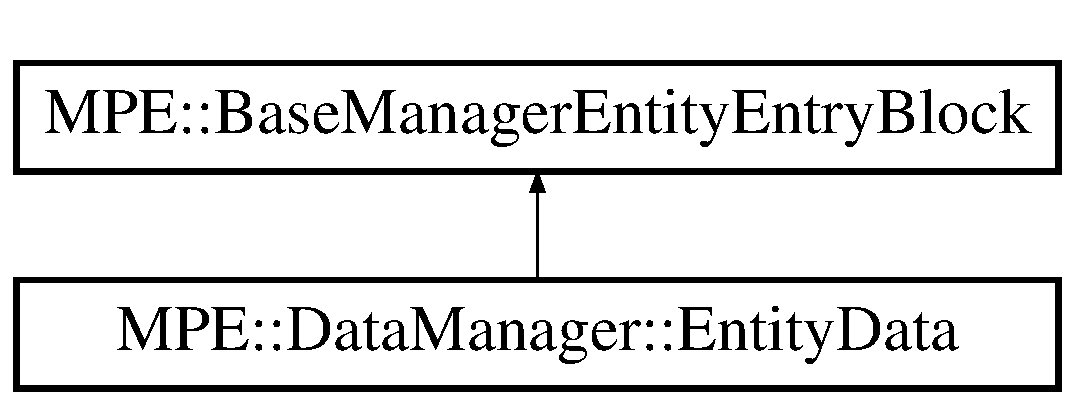
\includegraphics[height=2.000000cm]{struct_m_p_e_1_1_base_manager_entity_entry_block}
\end{center}
\end{figure}
\subsection*{Public Attributes}
\begin{DoxyCompactItemize}
\item 
uint32\+\_\+t \hyperlink{struct_m_p_e_1_1_base_manager_entity_entry_block_a9bb99ec160ea2058b700023dd7b05d78}{used} = 0
\item 
uint32\+\_\+t \hyperlink{struct_m_p_e_1_1_base_manager_entity_entry_block_a9a3b521d536a0650656c6ffd58868a56}{allocated} = 0
\item 
void $\ast$ \hyperlink{struct_m_p_e_1_1_base_manager_entity_entry_block_a474a83fa9930cbdcd6b4da102ae2b366}{buffer} = nullptr
\item 
\hyperlink{struct_m_p_e_1_1_entity}{Entity} $\ast$ \hyperlink{struct_m_p_e_1_1_base_manager_entity_entry_block_a6eddce97e38561fc4a22b5610ad3123c}{entity}
\end{DoxyCompactItemize}


\subsection{Detailed Description}
The memory where the data for each entity entry is held. 

Each array has the same number of entires and are concatenated in the memory block. 

\subsection{Member Data Documentation}
\mbox{\Hypertarget{struct_m_p_e_1_1_base_manager_entity_entry_block_a9a3b521d536a0650656c6ffd58868a56}\label{struct_m_p_e_1_1_base_manager_entity_entry_block_a9a3b521d536a0650656c6ffd58868a56}} 
\index{M\+P\+E\+::\+Base\+Manager\+Entity\+Entry\+Block@{M\+P\+E\+::\+Base\+Manager\+Entity\+Entry\+Block}!allocated@{allocated}}
\index{allocated@{allocated}!M\+P\+E\+::\+Base\+Manager\+Entity\+Entry\+Block@{M\+P\+E\+::\+Base\+Manager\+Entity\+Entry\+Block}}
\subsubsection{\texorpdfstring{allocated}{allocated}}
{\footnotesize\ttfamily uint32\+\_\+t M\+P\+E\+::\+Base\+Manager\+Entity\+Entry\+Block\+::allocated = 0}

Currently allocated entires in the block \mbox{\Hypertarget{struct_m_p_e_1_1_base_manager_entity_entry_block_a474a83fa9930cbdcd6b4da102ae2b366}\label{struct_m_p_e_1_1_base_manager_entity_entry_block_a474a83fa9930cbdcd6b4da102ae2b366}} 
\index{M\+P\+E\+::\+Base\+Manager\+Entity\+Entry\+Block@{M\+P\+E\+::\+Base\+Manager\+Entity\+Entry\+Block}!buffer@{buffer}}
\index{buffer@{buffer}!M\+P\+E\+::\+Base\+Manager\+Entity\+Entry\+Block@{M\+P\+E\+::\+Base\+Manager\+Entity\+Entry\+Block}}
\subsubsection{\texorpdfstring{buffer}{buffer}}
{\footnotesize\ttfamily void$\ast$ M\+P\+E\+::\+Base\+Manager\+Entity\+Entry\+Block\+::buffer = nullptr}

Pointer to the memory block \mbox{\Hypertarget{struct_m_p_e_1_1_base_manager_entity_entry_block_a6eddce97e38561fc4a22b5610ad3123c}\label{struct_m_p_e_1_1_base_manager_entity_entry_block_a6eddce97e38561fc4a22b5610ad3123c}} 
\index{M\+P\+E\+::\+Base\+Manager\+Entity\+Entry\+Block@{M\+P\+E\+::\+Base\+Manager\+Entity\+Entry\+Block}!entity@{entity}}
\index{entity@{entity}!M\+P\+E\+::\+Base\+Manager\+Entity\+Entry\+Block@{M\+P\+E\+::\+Base\+Manager\+Entity\+Entry\+Block}}
\subsubsection{\texorpdfstring{entity}{entity}}
{\footnotesize\ttfamily \hyperlink{struct_m_p_e_1_1_entity}{Entity}$\ast$ M\+P\+E\+::\+Base\+Manager\+Entity\+Entry\+Block\+::entity}

Stores the entity the entry is assigned to \mbox{\Hypertarget{struct_m_p_e_1_1_base_manager_entity_entry_block_a9bb99ec160ea2058b700023dd7b05d78}\label{struct_m_p_e_1_1_base_manager_entity_entry_block_a9bb99ec160ea2058b700023dd7b05d78}} 
\index{M\+P\+E\+::\+Base\+Manager\+Entity\+Entry\+Block@{M\+P\+E\+::\+Base\+Manager\+Entity\+Entry\+Block}!used@{used}}
\index{used@{used}!M\+P\+E\+::\+Base\+Manager\+Entity\+Entry\+Block@{M\+P\+E\+::\+Base\+Manager\+Entity\+Entry\+Block}}
\subsubsection{\texorpdfstring{used}{used}}
{\footnotesize\ttfamily uint32\+\_\+t M\+P\+E\+::\+Base\+Manager\+Entity\+Entry\+Block\+::used = 0}

Currently used entires in the block 

The documentation for this struct was generated from the following file\+:\begin{DoxyCompactItemize}
\item 
\hyperlink{_manager_8h}{Manager.\+h}\end{DoxyCompactItemize}

\hypertarget{struct_m_p_e_1_1_data_manager_1_1_data}{}\section{M\+PE\+:\+:Data\+Manager\+:\+:Data Struct Reference}
\label{struct_m_p_e_1_1_data_manager_1_1_data}\index{M\+P\+E\+::\+Data\+Manager\+::\+Data@{M\+P\+E\+::\+Data\+Manager\+::\+Data}}


Used for indexing the strings and other growing datatypes in the value\+\_\+buffer.  


\subsection*{Public Attributes}
\begin{DoxyCompactItemize}
\item 
uint16\+\_\+t \hyperlink{struct_m_p_e_1_1_data_manager_1_1_data_a453a2aeeef871f6d9d7d9fb8c1f74f05}{offset}
\item 
uint16\+\_\+t \hyperlink{struct_m_p_e_1_1_data_manager_1_1_data_af32b0baab1caac2b8398e75bc50a5f90}{size}
\end{DoxyCompactItemize}


\subsection{Detailed Description}
Used for indexing the strings and other growing datatypes in the value\+\_\+buffer. 

\subsection{Member Data Documentation}
\mbox{\Hypertarget{struct_m_p_e_1_1_data_manager_1_1_data_a453a2aeeef871f6d9d7d9fb8c1f74f05}\label{struct_m_p_e_1_1_data_manager_1_1_data_a453a2aeeef871f6d9d7d9fb8c1f74f05}} 
\index{M\+P\+E\+::\+Data\+Manager\+::\+Data@{M\+P\+E\+::\+Data\+Manager\+::\+Data}!offset@{offset}}
\index{offset@{offset}!M\+P\+E\+::\+Data\+Manager\+::\+Data@{M\+P\+E\+::\+Data\+Manager\+::\+Data}}
\subsubsection{\texorpdfstring{offset}{offset}}
{\footnotesize\ttfamily uint16\+\_\+t M\+P\+E\+::\+Data\+Manager\+::\+Data\+::offset}

\mbox{\Hypertarget{struct_m_p_e_1_1_data_manager_1_1_data_af32b0baab1caac2b8398e75bc50a5f90}\label{struct_m_p_e_1_1_data_manager_1_1_data_af32b0baab1caac2b8398e75bc50a5f90}} 
\index{M\+P\+E\+::\+Data\+Manager\+::\+Data@{M\+P\+E\+::\+Data\+Manager\+::\+Data}!size@{size}}
\index{size@{size}!M\+P\+E\+::\+Data\+Manager\+::\+Data@{M\+P\+E\+::\+Data\+Manager\+::\+Data}}
\subsubsection{\texorpdfstring{size}{size}}
{\footnotesize\ttfamily uint16\+\_\+t M\+P\+E\+::\+Data\+Manager\+::\+Data\+::size}



The documentation for this struct was generated from the following file\+:\begin{DoxyCompactItemize}
\item 
\hyperlink{_data_manager_8h}{Data\+Manager.\+h}\end{DoxyCompactItemize}

\hypertarget{struct_profiler_1_1_data}{}\section{Profiler\+:\+:Data Struct Reference}
\label{struct_profiler_1_1_data}\index{Profiler\+::\+Data@{Profiler\+::\+Data}}


{\ttfamily \#include $<$Profiler.\+h$>$}

\subsection*{Public Member Functions}
\begin{DoxyCompactItemize}
\item 
\hyperlink{struct_profiler_1_1_data_a948384dc5a585b604993a336227946d3}{Data} ()
\item 
\hyperlink{struct_profiler_1_1_data_a67dd48e639f8837ce3837180997f1fb5}{Data} (\hyperlink{struct_profiler_1_1_data}{Data} $\ast$\hyperlink{struct_profiler_1_1_data_a03fc44b9847c501d013edd119e9e2883}{parent}, const char $\ast$\hyperlink{struct_profiler_1_1_data_a7ba86ce73c788e68ac563f5dd2b7cf0e}{function\+Name})
\item 
\hyperlink{struct_profiler_1_1_data_a37cc05a58760958fe799a8bca8557c3f}{$\sim$\+Data} ()
\item 
const void \hyperlink{struct_profiler_1_1_data_af9bd89654595106b06b37bdfb1fd918f}{dump} (std\+::stringstream \&out)
\end{DoxyCompactItemize}
\subsection*{Public Attributes}
\begin{DoxyCompactItemize}
\item 
\hyperlink{struct_profiler_1_1_data}{Data} $\ast$ \hyperlink{struct_profiler_1_1_data_a03fc44b9847c501d013edd119e9e2883}{parent}
\item 
std\+::string \hyperlink{struct_profiler_1_1_data_a7ba86ce73c788e68ac563f5dd2b7cf0e}{function\+Name}
\item 
uint64\+\_\+t \hyperlink{struct_profiler_1_1_data_a0b2089e9dd5738281e01baa681b4e542}{times\+Called}
\item 
double \hyperlink{struct_profiler_1_1_data_a19d4cb0603046e7463c6dee9db916194}{time\+Spent}
\item 
std\+::chrono\+::high\+\_\+resolution\+\_\+clock\+::time\+\_\+point \hyperlink{struct_profiler_1_1_data_afbbb2195e44ec620890e389db3963afc}{time\+Start}
\item 
std\+::map$<$ uint64\+\_\+t, \hyperlink{struct_profiler_1_1_data}{Data} $\ast$ $>$ \hyperlink{struct_profiler_1_1_data_a5ca61fdcbac716347974f8dd71f95625}{children}
\end{DoxyCompactItemize}


\subsection{Constructor \& Destructor Documentation}
\mbox{\Hypertarget{struct_profiler_1_1_data_a948384dc5a585b604993a336227946d3}\label{struct_profiler_1_1_data_a948384dc5a585b604993a336227946d3}} 
\index{Profiler\+::\+Data@{Profiler\+::\+Data}!Data@{Data}}
\index{Data@{Data}!Profiler\+::\+Data@{Profiler\+::\+Data}}
\subsubsection{\texorpdfstring{Data()}{Data()}\hspace{0.1cm}{\footnotesize\ttfamily [1/2]}}
{\footnotesize\ttfamily Profiler\+::\+Data\+::\+Data (\begin{DoxyParamCaption}{ }\end{DoxyParamCaption})\hspace{0.3cm}{\ttfamily [inline]}}

\mbox{\Hypertarget{struct_profiler_1_1_data_a67dd48e639f8837ce3837180997f1fb5}\label{struct_profiler_1_1_data_a67dd48e639f8837ce3837180997f1fb5}} 
\index{Profiler\+::\+Data@{Profiler\+::\+Data}!Data@{Data}}
\index{Data@{Data}!Profiler\+::\+Data@{Profiler\+::\+Data}}
\subsubsection{\texorpdfstring{Data()}{Data()}\hspace{0.1cm}{\footnotesize\ttfamily [2/2]}}
{\footnotesize\ttfamily Profiler\+::\+Data\+::\+Data (\begin{DoxyParamCaption}\item[{\hyperlink{struct_profiler_1_1_data}{Data} $\ast$}]{parent,  }\item[{const char $\ast$}]{function\+Name }\end{DoxyParamCaption})\hspace{0.3cm}{\ttfamily [inline]}}

\mbox{\Hypertarget{struct_profiler_1_1_data_a37cc05a58760958fe799a8bca8557c3f}\label{struct_profiler_1_1_data_a37cc05a58760958fe799a8bca8557c3f}} 
\index{Profiler\+::\+Data@{Profiler\+::\+Data}!````~Data@{$\sim$\+Data}}
\index{````~Data@{$\sim$\+Data}!Profiler\+::\+Data@{Profiler\+::\+Data}}
\subsubsection{\texorpdfstring{$\sim$\+Data()}{~Data()}}
{\footnotesize\ttfamily Profiler\+::\+Data\+::$\sim$\+Data (\begin{DoxyParamCaption}{ }\end{DoxyParamCaption})\hspace{0.3cm}{\ttfamily [inline]}}



\subsection{Member Function Documentation}
\mbox{\Hypertarget{struct_profiler_1_1_data_af9bd89654595106b06b37bdfb1fd918f}\label{struct_profiler_1_1_data_af9bd89654595106b06b37bdfb1fd918f}} 
\index{Profiler\+::\+Data@{Profiler\+::\+Data}!dump@{dump}}
\index{dump@{dump}!Profiler\+::\+Data@{Profiler\+::\+Data}}
\subsubsection{\texorpdfstring{dump()}{dump()}}
{\footnotesize\ttfamily const void Profiler\+::\+Data\+::dump (\begin{DoxyParamCaption}\item[{std\+::stringstream \&}]{out }\end{DoxyParamCaption})}



\subsection{Member Data Documentation}
\mbox{\Hypertarget{struct_profiler_1_1_data_a5ca61fdcbac716347974f8dd71f95625}\label{struct_profiler_1_1_data_a5ca61fdcbac716347974f8dd71f95625}} 
\index{Profiler\+::\+Data@{Profiler\+::\+Data}!children@{children}}
\index{children@{children}!Profiler\+::\+Data@{Profiler\+::\+Data}}
\subsubsection{\texorpdfstring{children}{children}}
{\footnotesize\ttfamily std\+::map$<$uint64\+\_\+t, \hyperlink{struct_profiler_1_1_data}{Data}$\ast$$>$ Profiler\+::\+Data\+::children}

\mbox{\Hypertarget{struct_profiler_1_1_data_a7ba86ce73c788e68ac563f5dd2b7cf0e}\label{struct_profiler_1_1_data_a7ba86ce73c788e68ac563f5dd2b7cf0e}} 
\index{Profiler\+::\+Data@{Profiler\+::\+Data}!function\+Name@{function\+Name}}
\index{function\+Name@{function\+Name}!Profiler\+::\+Data@{Profiler\+::\+Data}}
\subsubsection{\texorpdfstring{function\+Name}{functionName}}
{\footnotesize\ttfamily std\+::string Profiler\+::\+Data\+::function\+Name}

\mbox{\Hypertarget{struct_profiler_1_1_data_a03fc44b9847c501d013edd119e9e2883}\label{struct_profiler_1_1_data_a03fc44b9847c501d013edd119e9e2883}} 
\index{Profiler\+::\+Data@{Profiler\+::\+Data}!parent@{parent}}
\index{parent@{parent}!Profiler\+::\+Data@{Profiler\+::\+Data}}
\subsubsection{\texorpdfstring{parent}{parent}}
{\footnotesize\ttfamily \hyperlink{struct_profiler_1_1_data}{Data}$\ast$ Profiler\+::\+Data\+::parent}

\mbox{\Hypertarget{struct_profiler_1_1_data_a0b2089e9dd5738281e01baa681b4e542}\label{struct_profiler_1_1_data_a0b2089e9dd5738281e01baa681b4e542}} 
\index{Profiler\+::\+Data@{Profiler\+::\+Data}!times\+Called@{times\+Called}}
\index{times\+Called@{times\+Called}!Profiler\+::\+Data@{Profiler\+::\+Data}}
\subsubsection{\texorpdfstring{times\+Called}{timesCalled}}
{\footnotesize\ttfamily uint64\+\_\+t Profiler\+::\+Data\+::times\+Called}

\mbox{\Hypertarget{struct_profiler_1_1_data_a19d4cb0603046e7463c6dee9db916194}\label{struct_profiler_1_1_data_a19d4cb0603046e7463c6dee9db916194}} 
\index{Profiler\+::\+Data@{Profiler\+::\+Data}!time\+Spent@{time\+Spent}}
\index{time\+Spent@{time\+Spent}!Profiler\+::\+Data@{Profiler\+::\+Data}}
\subsubsection{\texorpdfstring{time\+Spent}{timeSpent}}
{\footnotesize\ttfamily double Profiler\+::\+Data\+::time\+Spent}

\mbox{\Hypertarget{struct_profiler_1_1_data_afbbb2195e44ec620890e389db3963afc}\label{struct_profiler_1_1_data_afbbb2195e44ec620890e389db3963afc}} 
\index{Profiler\+::\+Data@{Profiler\+::\+Data}!time\+Start@{time\+Start}}
\index{time\+Start@{time\+Start}!Profiler\+::\+Data@{Profiler\+::\+Data}}
\subsubsection{\texorpdfstring{time\+Start}{timeStart}}
{\footnotesize\ttfamily std\+::chrono\+::high\+\_\+resolution\+\_\+clock\+::time\+\_\+point Profiler\+::\+Data\+::time\+Start}



The documentation for this struct was generated from the following file\+:\begin{DoxyCompactItemize}
\item 
\hyperlink{_profiler_8h}{Profiler.\+h}\end{DoxyCompactItemize}

\hypertarget{struct_m_p_e_1_1_data_manager_1_1_data_buffer}{}\section{M\+PE\+:\+:Data\+Manager\+:\+:Data\+Buffer Struct Reference}
\label{struct_m_p_e_1_1_data_manager_1_1_data_buffer}\index{M\+P\+E\+::\+Data\+Manager\+::\+Data\+Buffer@{M\+P\+E\+::\+Data\+Manager\+::\+Data\+Buffer}}


Struct for keeping track of the data entries an \hyperlink{struct_m_p_e_1_1_entity}{Entity} has been given.  


\subsection*{Public Member Functions}
\begin{DoxyCompactItemize}
\item 
\hyperlink{struct_m_p_e_1_1_data_manager_1_1_data_buffer_a85b5e0404f7e7bd6a2e8553e4977fcf6}{Data\+Buffer} ()
\item 
\hyperlink{struct_m_p_e_1_1_data_manager_1_1_data_buffer_ab733041fb29f94e89140b54f20771d4d}{$\sim$\+Data\+Buffer} ()
\item 
const void \hyperlink{struct_m_p_e_1_1_data_manager_1_1_data_buffer_ad69fcbc429f31ea23b2fdb4cf3f1db47}{Allocate} (size\+\_\+t size)
\begin{DoxyCompactList}\small\item\em Grow the entry buffer. \end{DoxyCompactList}\item 
const void \hyperlink{struct_m_p_e_1_1_data_manager_1_1_data_buffer_a89e5af3756f1359588936a3adc5c4b03}{Allocate\+And\+Resize\+Header} (size\+\_\+t size)
\begin{DoxyCompactList}\small\item\em Grow the entry buffer and copy the header immediately. \end{DoxyCompactList}\item 
const void \hyperlink{struct_m_p_e_1_1_data_manager_1_1_data_buffer_aa0c025d4f28747a2168748f8a492928f}{Header\+Resize} ()
\begin{DoxyCompactList}\small\item\em Grow the header. \end{DoxyCompactList}\end{DoxyCompactItemize}
\subsection*{Public Attributes}
\begin{DoxyCompactItemize}
\item 
void $\ast$ \hyperlink{struct_m_p_e_1_1_data_manager_1_1_data_buffer_afc54918e931e50e7b6491deb34aaad42}{data}
\item 
size\+\_\+t \hyperlink{struct_m_p_e_1_1_data_manager_1_1_data_buffer_ae239cb6309b020933fb4d158e7237a66}{capacity}
\item 
\hyperlink{struct_m_p_e_1_1_data_manager_1_1_entry_header}{Entry\+Header} \hyperlink{struct_m_p_e_1_1_data_manager_1_1_data_buffer_a392083d42f4f007a4c58dc2dd722d7f4}{header}
\item 
\hyperlink{struct_m_p_e_1_1_data_manager_1_1_value___buffer}{Value\+\_\+\+Buffer} \hyperlink{struct_m_p_e_1_1_data_manager_1_1_data_buffer_a27dfc55c4ae7fa07df7011e6232b982a}{v\+\_\+buffer}
\end{DoxyCompactItemize}


\subsection{Detailed Description}
Struct for keeping track of the data entries an \hyperlink{struct_m_p_e_1_1_entity}{Entity} has been given. 

The databuffer stores the header on the left side and the value\+\_\+buffer on the right side. When the buffers meet the size is increased. 

\subsection{Constructor \& Destructor Documentation}
\mbox{\Hypertarget{struct_m_p_e_1_1_data_manager_1_1_data_buffer_a85b5e0404f7e7bd6a2e8553e4977fcf6}\label{struct_m_p_e_1_1_data_manager_1_1_data_buffer_a85b5e0404f7e7bd6a2e8553e4977fcf6}} 
\index{M\+P\+E\+::\+Data\+Manager\+::\+Data\+Buffer@{M\+P\+E\+::\+Data\+Manager\+::\+Data\+Buffer}!Data\+Buffer@{Data\+Buffer}}
\index{Data\+Buffer@{Data\+Buffer}!M\+P\+E\+::\+Data\+Manager\+::\+Data\+Buffer@{M\+P\+E\+::\+Data\+Manager\+::\+Data\+Buffer}}
\subsubsection{\texorpdfstring{Data\+Buffer()}{DataBuffer()}}
{\footnotesize\ttfamily M\+P\+E\+::\+Data\+Manager\+::\+Data\+Buffer\+::\+Data\+Buffer (\begin{DoxyParamCaption}{ }\end{DoxyParamCaption})}

\mbox{\Hypertarget{struct_m_p_e_1_1_data_manager_1_1_data_buffer_ab733041fb29f94e89140b54f20771d4d}\label{struct_m_p_e_1_1_data_manager_1_1_data_buffer_ab733041fb29f94e89140b54f20771d4d}} 
\index{M\+P\+E\+::\+Data\+Manager\+::\+Data\+Buffer@{M\+P\+E\+::\+Data\+Manager\+::\+Data\+Buffer}!````~Data\+Buffer@{$\sim$\+Data\+Buffer}}
\index{````~Data\+Buffer@{$\sim$\+Data\+Buffer}!M\+P\+E\+::\+Data\+Manager\+::\+Data\+Buffer@{M\+P\+E\+::\+Data\+Manager\+::\+Data\+Buffer}}
\subsubsection{\texorpdfstring{$\sim$\+Data\+Buffer()}{~DataBuffer()}}
{\footnotesize\ttfamily M\+P\+E\+::\+Data\+Manager\+::\+Data\+Buffer\+::$\sim$\+Data\+Buffer (\begin{DoxyParamCaption}{ }\end{DoxyParamCaption})}



\subsection{Member Function Documentation}
\mbox{\Hypertarget{struct_m_p_e_1_1_data_manager_1_1_data_buffer_ad69fcbc429f31ea23b2fdb4cf3f1db47}\label{struct_m_p_e_1_1_data_manager_1_1_data_buffer_ad69fcbc429f31ea23b2fdb4cf3f1db47}} 
\index{M\+P\+E\+::\+Data\+Manager\+::\+Data\+Buffer@{M\+P\+E\+::\+Data\+Manager\+::\+Data\+Buffer}!Allocate@{Allocate}}
\index{Allocate@{Allocate}!M\+P\+E\+::\+Data\+Manager\+::\+Data\+Buffer@{M\+P\+E\+::\+Data\+Manager\+::\+Data\+Buffer}}
\subsubsection{\texorpdfstring{Allocate()}{Allocate()}}
{\footnotesize\ttfamily const void M\+P\+E\+::\+Data\+Manager\+::\+Data\+Buffer\+::\+Allocate (\begin{DoxyParamCaption}\item[{size\+\_\+t}]{size }\end{DoxyParamCaption})}



Grow the entry buffer. 

\mbox{\Hypertarget{struct_m_p_e_1_1_data_manager_1_1_data_buffer_a89e5af3756f1359588936a3adc5c4b03}\label{struct_m_p_e_1_1_data_manager_1_1_data_buffer_a89e5af3756f1359588936a3adc5c4b03}} 
\index{M\+P\+E\+::\+Data\+Manager\+::\+Data\+Buffer@{M\+P\+E\+::\+Data\+Manager\+::\+Data\+Buffer}!Allocate\+And\+Resize\+Header@{Allocate\+And\+Resize\+Header}}
\index{Allocate\+And\+Resize\+Header@{Allocate\+And\+Resize\+Header}!M\+P\+E\+::\+Data\+Manager\+::\+Data\+Buffer@{M\+P\+E\+::\+Data\+Manager\+::\+Data\+Buffer}}
\subsubsection{\texorpdfstring{Allocate\+And\+Resize\+Header()}{AllocateAndResizeHeader()}}
{\footnotesize\ttfamily const void M\+P\+E\+::\+Data\+Manager\+::\+Data\+Buffer\+::\+Allocate\+And\+Resize\+Header (\begin{DoxyParamCaption}\item[{size\+\_\+t}]{size }\end{DoxyParamCaption})}



Grow the entry buffer and copy the header immediately. 

\mbox{\Hypertarget{struct_m_p_e_1_1_data_manager_1_1_data_buffer_aa0c025d4f28747a2168748f8a492928f}\label{struct_m_p_e_1_1_data_manager_1_1_data_buffer_aa0c025d4f28747a2168748f8a492928f}} 
\index{M\+P\+E\+::\+Data\+Manager\+::\+Data\+Buffer@{M\+P\+E\+::\+Data\+Manager\+::\+Data\+Buffer}!Header\+Resize@{Header\+Resize}}
\index{Header\+Resize@{Header\+Resize}!M\+P\+E\+::\+Data\+Manager\+::\+Data\+Buffer@{M\+P\+E\+::\+Data\+Manager\+::\+Data\+Buffer}}
\subsubsection{\texorpdfstring{Header\+Resize()}{HeaderResize()}}
{\footnotesize\ttfamily const void M\+P\+E\+::\+Data\+Manager\+::\+Data\+Buffer\+::\+Header\+Resize (\begin{DoxyParamCaption}{ }\end{DoxyParamCaption})}



Grow the header. 



\subsection{Member Data Documentation}
\mbox{\Hypertarget{struct_m_p_e_1_1_data_manager_1_1_data_buffer_ae239cb6309b020933fb4d158e7237a66}\label{struct_m_p_e_1_1_data_manager_1_1_data_buffer_ae239cb6309b020933fb4d158e7237a66}} 
\index{M\+P\+E\+::\+Data\+Manager\+::\+Data\+Buffer@{M\+P\+E\+::\+Data\+Manager\+::\+Data\+Buffer}!capacity@{capacity}}
\index{capacity@{capacity}!M\+P\+E\+::\+Data\+Manager\+::\+Data\+Buffer@{M\+P\+E\+::\+Data\+Manager\+::\+Data\+Buffer}}
\subsubsection{\texorpdfstring{capacity}{capacity}}
{\footnotesize\ttfamily size\+\_\+t M\+P\+E\+::\+Data\+Manager\+::\+Data\+Buffer\+::capacity}

This capacity is in bytes!!! \mbox{\Hypertarget{struct_m_p_e_1_1_data_manager_1_1_data_buffer_afc54918e931e50e7b6491deb34aaad42}\label{struct_m_p_e_1_1_data_manager_1_1_data_buffer_afc54918e931e50e7b6491deb34aaad42}} 
\index{M\+P\+E\+::\+Data\+Manager\+::\+Data\+Buffer@{M\+P\+E\+::\+Data\+Manager\+::\+Data\+Buffer}!data@{data}}
\index{data@{data}!M\+P\+E\+::\+Data\+Manager\+::\+Data\+Buffer@{M\+P\+E\+::\+Data\+Manager\+::\+Data\+Buffer}}
\subsubsection{\texorpdfstring{data}{data}}
{\footnotesize\ttfamily void$\ast$ M\+P\+E\+::\+Data\+Manager\+::\+Data\+Buffer\+::data}

\mbox{\Hypertarget{struct_m_p_e_1_1_data_manager_1_1_data_buffer_a392083d42f4f007a4c58dc2dd722d7f4}\label{struct_m_p_e_1_1_data_manager_1_1_data_buffer_a392083d42f4f007a4c58dc2dd722d7f4}} 
\index{M\+P\+E\+::\+Data\+Manager\+::\+Data\+Buffer@{M\+P\+E\+::\+Data\+Manager\+::\+Data\+Buffer}!header@{header}}
\index{header@{header}!M\+P\+E\+::\+Data\+Manager\+::\+Data\+Buffer@{M\+P\+E\+::\+Data\+Manager\+::\+Data\+Buffer}}
\subsubsection{\texorpdfstring{header}{header}}
{\footnotesize\ttfamily \hyperlink{struct_m_p_e_1_1_data_manager_1_1_entry_header}{Entry\+Header} M\+P\+E\+::\+Data\+Manager\+::\+Data\+Buffer\+::header}

\mbox{\Hypertarget{struct_m_p_e_1_1_data_manager_1_1_data_buffer_a27dfc55c4ae7fa07df7011e6232b982a}\label{struct_m_p_e_1_1_data_manager_1_1_data_buffer_a27dfc55c4ae7fa07df7011e6232b982a}} 
\index{M\+P\+E\+::\+Data\+Manager\+::\+Data\+Buffer@{M\+P\+E\+::\+Data\+Manager\+::\+Data\+Buffer}!v\+\_\+buffer@{v\+\_\+buffer}}
\index{v\+\_\+buffer@{v\+\_\+buffer}!M\+P\+E\+::\+Data\+Manager\+::\+Data\+Buffer@{M\+P\+E\+::\+Data\+Manager\+::\+Data\+Buffer}}
\subsubsection{\texorpdfstring{v\+\_\+buffer}{v\_buffer}}
{\footnotesize\ttfamily \hyperlink{struct_m_p_e_1_1_data_manager_1_1_value___buffer}{Value\+\_\+\+Buffer} M\+P\+E\+::\+Data\+Manager\+::\+Data\+Buffer\+::v\+\_\+buffer}



The documentation for this struct was generated from the following files\+:\begin{DoxyCompactItemize}
\item 
\hyperlink{_data_manager_8h}{Data\+Manager.\+h}\item 
\hyperlink{_data_manager_8cpp}{Data\+Manager.\+cpp}\end{DoxyCompactItemize}

\hypertarget{class_m_p_e_1_1_data_manager}{}\section{M\+PE\+:\+:Data\+Manager Class Reference}
\label{class_m_p_e_1_1_data_manager}\index{M\+P\+E\+::\+Data\+Manager@{M\+P\+E\+::\+Data\+Manager}}


The \hyperlink{class_m_p_e_1_1_data_manager}{Data\+Manager} is used to associate basic datatypes to an entity.  




{\ttfamily \#include $<$Data\+Manager.\+h$>$}

Inheritance diagram for M\+PE\+:\+:Data\+Manager\+:\begin{figure}[H]
\begin{center}
\leavevmode
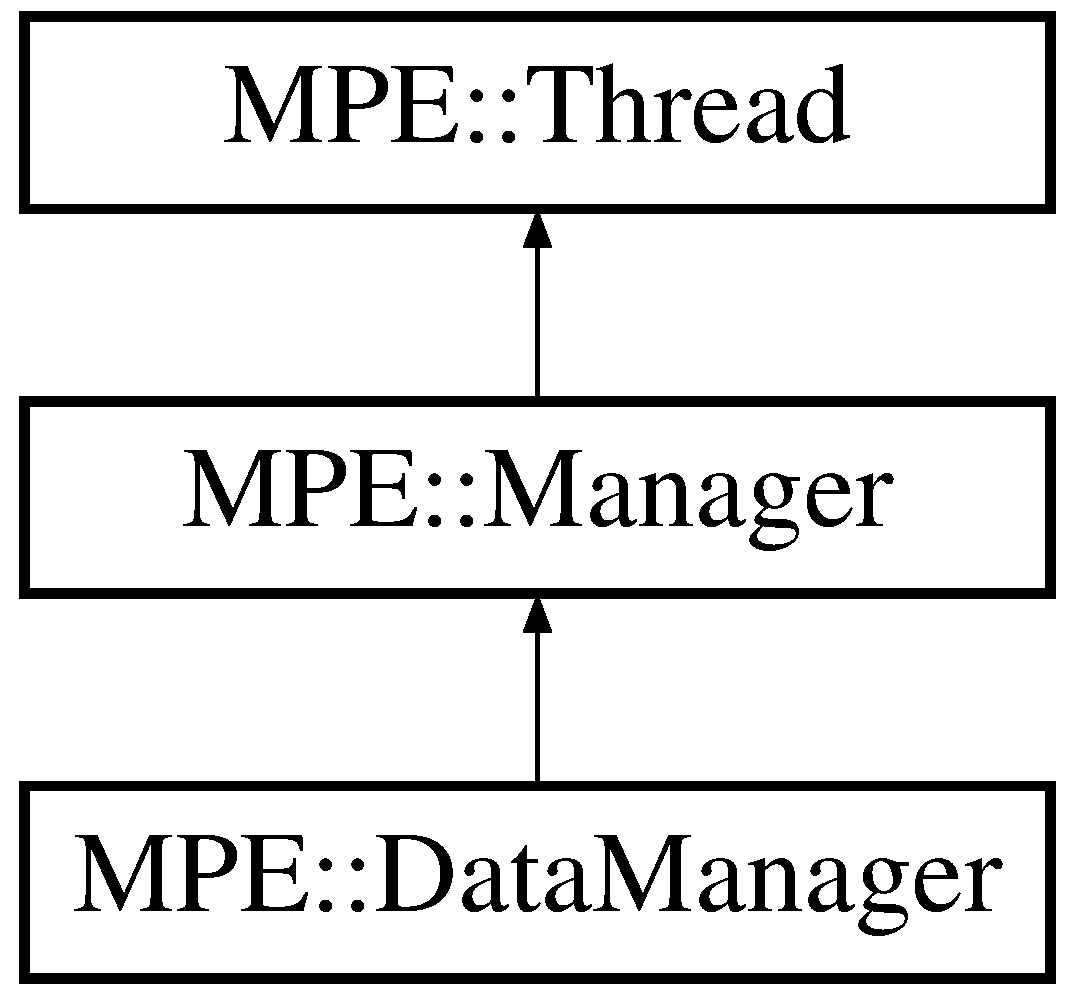
\includegraphics[height=3.000000cm]{class_m_p_e_1_1_data_manager}
\end{center}
\end{figure}
\subsection*{Classes}
\begin{DoxyCompactItemize}
\item 
struct \hyperlink{struct_m_p_e_1_1_data_manager_1_1_data}{Data}
\begin{DoxyCompactList}\small\item\em Used for indexing the strings and other growing datatypes in the value\+\_\+buffer. \end{DoxyCompactList}\item 
struct \hyperlink{struct_m_p_e_1_1_data_manager_1_1_data_buffer}{Data\+Buffer}
\begin{DoxyCompactList}\small\item\em Struct for keeping track of the data entries an \hyperlink{struct_m_p_e_1_1_entity}{Entity} has been given. \end{DoxyCompactList}\item 
struct \hyperlink{struct_m_p_e_1_1_data_manager_1_1_entity_data}{Entity\+Data}
\begin{DoxyCompactList}\small\item\em The managers \hyperlink{struct_m_p_e_1_1_entity}{Entity} entry block. \end{DoxyCompactList}\item 
struct \hyperlink{struct_m_p_e_1_1_data_manager_1_1_entry_header}{Entry\+Header}
\begin{DoxyCompactList}\small\item\em The header struct, used for keeping track of the data entries an \hyperlink{struct_m_p_e_1_1_entity}{Entity} has. \end{DoxyCompactList}\item 
struct \hyperlink{struct_m_p_e_1_1_data_manager_1_1_value}{Value}
\begin{DoxyCompactList}\small\item\em The value struct, this is where the data is stored. \end{DoxyCompactList}\item 
struct \hyperlink{struct_m_p_e_1_1_data_manager_1_1_value___buffer}{Value\+\_\+\+Buffer}
\begin{DoxyCompactList}\small\item\em Points to the next free spot in the value\+\_\+buffer. \end{DoxyCompactList}\end{DoxyCompactItemize}
\subsection*{Public Member Functions}
\begin{DoxyCompactItemize}
\item 
\hyperlink{class_m_p_e_1_1_data_manager_a1af39853286eeaf8850b9e326ea24205}{Data\+Manager} (\hyperlink{namespace_m_p_e_a16447295e3105bd2ba2a9ea303566175}{thread\+Identifier} identifier, uint8\+\_\+t frame\+Sync\+Time=16)
\item 
\hyperlink{class_m_p_e_1_1_data_manager_ab6bdecd89d27d69d790a864175f8cf52}{$\sim$\+Data\+Manager} ()
\item 
const void \hyperlink{class_m_p_e_1_1_data_manager_aa8d6f1ef687afb532d968a3c1a42f324}{Start} ()
\begin{DoxyCompactList}\small\item\em The main entry point for the thread. \end{DoxyCompactList}\end{DoxyCompactItemize}
\subsection*{Private Types}
\begin{DoxyCompactItemize}
\item 
enum \hyperlink{class_m_p_e_1_1_data_manager_aeebd98a9feed805f5ebd63276f003f5f}{Data\+Type} \+: uint8\+\_\+t \{ \hyperlink{class_m_p_e_1_1_data_manager_aeebd98a9feed805f5ebd63276f003f5faa97b2c144243b2b9d2c593ec268b62f5}{Data\+Type\+::\+B\+O\+OL}, 
\hyperlink{class_m_p_e_1_1_data_manager_aeebd98a9feed805f5ebd63276f003f5fae738c26bf4ce1037fa81b039a915cbf6}{Data\+Type\+::\+F\+L\+O\+AT}, 
\hyperlink{class_m_p_e_1_1_data_manager_aeebd98a9feed805f5ebd63276f003f5fa63b588d5559f64f89a416e656880b949}{Data\+Type\+::\+S\+T\+R\+I\+NG}
 \}\begin{DoxyCompactList}\small\item\em For the kinds of data that can be stored as an entry. \end{DoxyCompactList}
\end{DoxyCompactItemize}
\subsection*{Private Member Functions}
\begin{DoxyCompactItemize}
\item 
const void \hyperlink{class_m_p_e_1_1_data_manager_ad164b9613a36a5bbb70bb8aac700416a}{\+\_\+\+Create\+Data} (const \hyperlink{struct_m_p_e_1_1_entity}{Entity} \&entity)
\begin{DoxyCompactList}\small\item\em Register an \hyperlink{struct_m_p_e_1_1_entity}{Entity} entry. \end{DoxyCompactList}\item 
const void \hyperlink{class_m_p_e_1_1_data_manager_acfb97e38f7c66cb59769835554c43e82}{\+\_\+\+Allocate} (uint32\+\_\+t size)
\begin{DoxyCompactList}\small\item\em Allocate more memory. \end{DoxyCompactList}\item 
const void \hyperlink{class_m_p_e_1_1_data_manager_aac128f82ae3d0e37ce8afc46f493dc4b}{\+\_\+\+Destroy} (uint32\+\_\+t index)
\begin{DoxyCompactList}\small\item\em Delete an entry in the memory block. \end{DoxyCompactList}\end{DoxyCompactItemize}
\subsection*{Private Attributes}
\begin{DoxyCompactItemize}
\item 
\hyperlink{struct_m_p_e_1_1_data_manager_1_1_entity_data}{Entity\+Data} \hyperlink{class_m_p_e_1_1_data_manager_a7c31d54443c2ff3dc77e2bf392de09ef}{\+\_\+entity\+Entires}
\end{DoxyCompactItemize}
\subsection*{Additional Inherited Members}


\subsection{Detailed Description}
The \hyperlink{class_m_p_e_1_1_data_manager}{Data\+Manager} is used to associate basic datatypes to an entity. 

By sending a message to the data manager you can add one or more data entries to an entity. Each entry contains one \hyperlink{struct_m_p_e_1_1_data_manager_1_1_data_buffer}{Data\+Buffer}. In the beginning of the \hyperlink{struct_m_p_e_1_1_data_manager_1_1_data_buffer}{Data\+Buffer} the \hyperlink{struct_m_p_e_1_1_data_manager_1_1_entry_header}{Entry\+Header} is located(which contains the \hyperlink{struct_m_p_e_1_1_data_manager_1_1_value}{Value} for each Data\+Type entry. The strings are stored at the end of the \hyperlink{struct_m_p_e_1_1_data_manager_1_1_data_buffer}{Data\+Buffer}. \begin{DoxySeeAlso}{See also}
\hyperlink{class_m_p_e_1_1_data_manager_aeebd98a9feed805f5ebd63276f003f5f}{Data\+Type} 

\hyperlink{namespace_m_p_e_1_1_tag_1_1_data_manager}{Tag\+::\+Data\+Manager} 
\end{DoxySeeAlso}


\subsection{Member Enumeration Documentation}
\mbox{\Hypertarget{class_m_p_e_1_1_data_manager_aeebd98a9feed805f5ebd63276f003f5f}\label{class_m_p_e_1_1_data_manager_aeebd98a9feed805f5ebd63276f003f5f}} 
\index{M\+P\+E\+::\+Data\+Manager@{M\+P\+E\+::\+Data\+Manager}!Data\+Type@{Data\+Type}}
\index{Data\+Type@{Data\+Type}!M\+P\+E\+::\+Data\+Manager@{M\+P\+E\+::\+Data\+Manager}}
\subsubsection{\texorpdfstring{Data\+Type}{DataType}}
{\footnotesize\ttfamily enum \hyperlink{class_m_p_e_1_1_data_manager_aeebd98a9feed805f5ebd63276f003f5f}{M\+P\+E\+::\+Data\+Manager\+::\+Data\+Type} \+: uint8\+\_\+t\hspace{0.3cm}{\ttfamily [strong]}, {\ttfamily [private]}}



For the kinds of data that can be stored as an entry. 

\begin{DoxyEnumFields}{Enumerator}
\raisebox{\heightof{T}}[0pt][0pt]{\index{B\+O\+OL@{B\+O\+OL}!M\+P\+E\+::\+Data\+Manager@{M\+P\+E\+::\+Data\+Manager}}\index{M\+P\+E\+::\+Data\+Manager@{M\+P\+E\+::\+Data\+Manager}!B\+O\+OL@{B\+O\+OL}}}\mbox{\Hypertarget{class_m_p_e_1_1_data_manager_aeebd98a9feed805f5ebd63276f003f5faa97b2c144243b2b9d2c593ec268b62f5}\label{class_m_p_e_1_1_data_manager_aeebd98a9feed805f5ebd63276f003f5faa97b2c144243b2b9d2c593ec268b62f5}} 
B\+O\+OL&\\
\hline

\raisebox{\heightof{T}}[0pt][0pt]{\index{F\+L\+O\+AT@{F\+L\+O\+AT}!M\+P\+E\+::\+Data\+Manager@{M\+P\+E\+::\+Data\+Manager}}\index{M\+P\+E\+::\+Data\+Manager@{M\+P\+E\+::\+Data\+Manager}!F\+L\+O\+AT@{F\+L\+O\+AT}}}\mbox{\Hypertarget{class_m_p_e_1_1_data_manager_aeebd98a9feed805f5ebd63276f003f5fae738c26bf4ce1037fa81b039a915cbf6}\label{class_m_p_e_1_1_data_manager_aeebd98a9feed805f5ebd63276f003f5fae738c26bf4ce1037fa81b039a915cbf6}} 
F\+L\+O\+AT&\\
\hline

\raisebox{\heightof{T}}[0pt][0pt]{\index{S\+T\+R\+I\+NG@{S\+T\+R\+I\+NG}!M\+P\+E\+::\+Data\+Manager@{M\+P\+E\+::\+Data\+Manager}}\index{M\+P\+E\+::\+Data\+Manager@{M\+P\+E\+::\+Data\+Manager}!S\+T\+R\+I\+NG@{S\+T\+R\+I\+NG}}}\mbox{\Hypertarget{class_m_p_e_1_1_data_manager_aeebd98a9feed805f5ebd63276f003f5fa63b588d5559f64f89a416e656880b949}\label{class_m_p_e_1_1_data_manager_aeebd98a9feed805f5ebd63276f003f5fa63b588d5559f64f89a416e656880b949}} 
S\+T\+R\+I\+NG&\\
\hline

\end{DoxyEnumFields}


\subsection{Constructor \& Destructor Documentation}
\mbox{\Hypertarget{class_m_p_e_1_1_data_manager_a1af39853286eeaf8850b9e326ea24205}\label{class_m_p_e_1_1_data_manager_a1af39853286eeaf8850b9e326ea24205}} 
\index{M\+P\+E\+::\+Data\+Manager@{M\+P\+E\+::\+Data\+Manager}!Data\+Manager@{Data\+Manager}}
\index{Data\+Manager@{Data\+Manager}!M\+P\+E\+::\+Data\+Manager@{M\+P\+E\+::\+Data\+Manager}}
\subsubsection{\texorpdfstring{Data\+Manager()}{DataManager()}}
{\footnotesize\ttfamily M\+P\+E\+::\+Data\+Manager\+::\+Data\+Manager (\begin{DoxyParamCaption}\item[{\hyperlink{namespace_m_p_e_a16447295e3105bd2ba2a9ea303566175}{thread\+Identifier}}]{identifier,  }\item[{uint8\+\_\+t}]{frame\+Sync\+Time = {\ttfamily 16} }\end{DoxyParamCaption})}

\mbox{\Hypertarget{class_m_p_e_1_1_data_manager_ab6bdecd89d27d69d790a864175f8cf52}\label{class_m_p_e_1_1_data_manager_ab6bdecd89d27d69d790a864175f8cf52}} 
\index{M\+P\+E\+::\+Data\+Manager@{M\+P\+E\+::\+Data\+Manager}!````~Data\+Manager@{$\sim$\+Data\+Manager}}
\index{````~Data\+Manager@{$\sim$\+Data\+Manager}!M\+P\+E\+::\+Data\+Manager@{M\+P\+E\+::\+Data\+Manager}}
\subsubsection{\texorpdfstring{$\sim$\+Data\+Manager()}{~DataManager()}}
{\footnotesize\ttfamily M\+P\+E\+::\+Data\+Manager\+::$\sim$\+Data\+Manager (\begin{DoxyParamCaption}{ }\end{DoxyParamCaption})}



\subsection{Member Function Documentation}
\mbox{\Hypertarget{class_m_p_e_1_1_data_manager_acfb97e38f7c66cb59769835554c43e82}\label{class_m_p_e_1_1_data_manager_acfb97e38f7c66cb59769835554c43e82}} 
\index{M\+P\+E\+::\+Data\+Manager@{M\+P\+E\+::\+Data\+Manager}!\+\_\+\+Allocate@{\+\_\+\+Allocate}}
\index{\+\_\+\+Allocate@{\+\_\+\+Allocate}!M\+P\+E\+::\+Data\+Manager@{M\+P\+E\+::\+Data\+Manager}}
\subsubsection{\texorpdfstring{\+\_\+\+Allocate()}{\_Allocate()}}
{\footnotesize\ttfamily const void M\+P\+E\+::\+Data\+Manager\+::\+\_\+\+Allocate (\begin{DoxyParamCaption}\item[{uint32\+\_\+t}]{size }\end{DoxyParamCaption})\hspace{0.3cm}{\ttfamily [private]}}



Allocate more memory. 

\mbox{\Hypertarget{class_m_p_e_1_1_data_manager_ad164b9613a36a5bbb70bb8aac700416a}\label{class_m_p_e_1_1_data_manager_ad164b9613a36a5bbb70bb8aac700416a}} 
\index{M\+P\+E\+::\+Data\+Manager@{M\+P\+E\+::\+Data\+Manager}!\+\_\+\+Create\+Data@{\+\_\+\+Create\+Data}}
\index{\+\_\+\+Create\+Data@{\+\_\+\+Create\+Data}!M\+P\+E\+::\+Data\+Manager@{M\+P\+E\+::\+Data\+Manager}}
\subsubsection{\texorpdfstring{\+\_\+\+Create\+Data()}{\_CreateData()}}
{\footnotesize\ttfamily const void M\+P\+E\+::\+Data\+Manager\+::\+\_\+\+Create\+Data (\begin{DoxyParamCaption}\item[{const \hyperlink{struct_m_p_e_1_1_entity}{Entity} \&}]{entity }\end{DoxyParamCaption})\hspace{0.3cm}{\ttfamily [private]}}



Register an \hyperlink{struct_m_p_e_1_1_entity}{Entity} entry. 

An \hyperlink{struct_m_p_e_1_1_entity}{Entity} need to be registered before any data can be associated with the \hyperlink{struct_m_p_e_1_1_entity}{Entity}. \mbox{\Hypertarget{class_m_p_e_1_1_data_manager_aac128f82ae3d0e37ce8afc46f493dc4b}\label{class_m_p_e_1_1_data_manager_aac128f82ae3d0e37ce8afc46f493dc4b}} 
\index{M\+P\+E\+::\+Data\+Manager@{M\+P\+E\+::\+Data\+Manager}!\+\_\+\+Destroy@{\+\_\+\+Destroy}}
\index{\+\_\+\+Destroy@{\+\_\+\+Destroy}!M\+P\+E\+::\+Data\+Manager@{M\+P\+E\+::\+Data\+Manager}}
\subsubsection{\texorpdfstring{\+\_\+\+Destroy()}{\_Destroy()}}
{\footnotesize\ttfamily const void M\+P\+E\+::\+Data\+Manager\+::\+\_\+\+Destroy (\begin{DoxyParamCaption}\item[{uint32\+\_\+t}]{index }\end{DoxyParamCaption})\hspace{0.3cm}{\ttfamily [private]}}



Delete an entry in the memory block. 

The deleted entry is replaced by the last in the block. \mbox{\Hypertarget{class_m_p_e_1_1_data_manager_aa8d6f1ef687afb532d968a3c1a42f324}\label{class_m_p_e_1_1_data_manager_aa8d6f1ef687afb532d968a3c1a42f324}} 
\index{M\+P\+E\+::\+Data\+Manager@{M\+P\+E\+::\+Data\+Manager}!Start@{Start}}
\index{Start@{Start}!M\+P\+E\+::\+Data\+Manager@{M\+P\+E\+::\+Data\+Manager}}
\subsubsection{\texorpdfstring{Start()}{Start()}}
{\footnotesize\ttfamily const void M\+P\+E\+::\+Data\+Manager\+::\+Start (\begin{DoxyParamCaption}{ }\end{DoxyParamCaption})\hspace{0.3cm}{\ttfamily [virtual]}}



The main entry point for the thread. 



Implements \hyperlink{class_m_p_e_1_1_thread_a1bd133a96ec27c868b6bb758e11c0691}{M\+P\+E\+::\+Thread}.



\subsection{Member Data Documentation}
\mbox{\Hypertarget{class_m_p_e_1_1_data_manager_a7c31d54443c2ff3dc77e2bf392de09ef}\label{class_m_p_e_1_1_data_manager_a7c31d54443c2ff3dc77e2bf392de09ef}} 
\index{M\+P\+E\+::\+Data\+Manager@{M\+P\+E\+::\+Data\+Manager}!\+\_\+entity\+Entires@{\+\_\+entity\+Entires}}
\index{\+\_\+entity\+Entires@{\+\_\+entity\+Entires}!M\+P\+E\+::\+Data\+Manager@{M\+P\+E\+::\+Data\+Manager}}
\subsubsection{\texorpdfstring{\+\_\+entity\+Entires}{\_entityEntires}}
{\footnotesize\ttfamily \hyperlink{struct_m_p_e_1_1_data_manager_1_1_entity_data}{Entity\+Data} M\+P\+E\+::\+Data\+Manager\+::\+\_\+entity\+Entires\hspace{0.3cm}{\ttfamily [private]}}

A reference pointer to avoid having to cast the basic datapointer all the time. 

The documentation for this class was generated from the following files\+:\begin{DoxyCompactItemize}
\item 
\hyperlink{_data_manager_8h}{Data\+Manager.\+h}\item 
\hyperlink{_data_manager_8cpp}{Data\+Manager.\+cpp}\end{DoxyCompactItemize}

\hypertarget{struct_m_p_e_1_1_entity}{}\section{M\+PE\+:\+:Entity Struct Reference}
\label{struct_m_p_e_1_1_entity}\index{M\+P\+E\+::\+Entity@{M\+P\+E\+::\+Entity}}


\hyperlink{struct_m_p_e_1_1_entity}{Entity} is essentially an id.  




{\ttfamily \#include $<$Entity.\+h$>$}

\subsection*{Public Member Functions}
\begin{DoxyCompactItemize}
\item 
\hyperlink{struct_m_p_e_1_1_entity_a7a748d33b99ad088cd933578ad4533f6}{Entity} ()
\begin{DoxyCompactList}\small\item\em Creates the entity. \end{DoxyCompactList}\item 
\hyperlink{struct_m_p_e_1_1_entity_acf0e7947c1814f2984de87590963360d}{Entity} (const uint64\+\_\+t \hyperlink{struct_m_p_e_1_1_entity_a04ff49ec80c37388b0e6a75cec860ceb}{ID})
\begin{DoxyCompactList}\small\item\em Creates the entity with a specified ID. \end{DoxyCompactList}\item 
\hyperlink{struct_m_p_e_1_1_entity_a985a1dae08ed4ab82e4a0ae2263cb4a7}{operator const uint64\+\_\+t} () const
\begin{DoxyCompactList}\small\item\em Conversion to uint64\+\_\+t. \end{DoxyCompactList}\item 
const \hyperlink{struct_m_p_e_1_1_entity}{Entity} \& \hyperlink{struct_m_p_e_1_1_entity_aa48771c026e87c391bff9e75d179b538}{operator=} (const uint64\+\_\+t \&other)
\item 
const \hyperlink{struct_m_p_e_1_1_entity}{Entity} \& \hyperlink{struct_m_p_e_1_1_entity_ad356d6b8c3df7cbd8dcc24dd1a3d718d}{operator=} (const \hyperlink{struct_m_p_e_1_1_entity}{Entity} \&other)
\item 
const bool \hyperlink{struct_m_p_e_1_1_entity_a587d74654df3a9be46403264c9bb016a}{operator==} (const \hyperlink{struct_m_p_e_1_1_entity}{Entity} \&other) const
\end{DoxyCompactItemize}
\subsection*{Public Attributes}
\begin{DoxyCompactItemize}
\item 
uint64\+\_\+t \hyperlink{struct_m_p_e_1_1_entity_a04ff49ec80c37388b0e6a75cec860ceb}{ID}
\end{DoxyCompactItemize}
\subsection*{Static Private Member Functions}
\begin{DoxyCompactItemize}
\item 
static const uint64\+\_\+t \hyperlink{struct_m_p_e_1_1_entity_a629768de1229b78f58ef62534fe74663}{Generate\+ID} ()
\end{DoxyCompactItemize}


\subsection{Detailed Description}
\hyperlink{struct_m_p_e_1_1_entity}{Entity} is essentially an id. 

\subsection{Constructor \& Destructor Documentation}
\mbox{\Hypertarget{struct_m_p_e_1_1_entity_a7a748d33b99ad088cd933578ad4533f6}\label{struct_m_p_e_1_1_entity_a7a748d33b99ad088cd933578ad4533f6}} 
\index{M\+P\+E\+::\+Entity@{M\+P\+E\+::\+Entity}!Entity@{Entity}}
\index{Entity@{Entity}!M\+P\+E\+::\+Entity@{M\+P\+E\+::\+Entity}}
\subsubsection{\texorpdfstring{Entity()}{Entity()}\hspace{0.1cm}{\footnotesize\ttfamily [1/2]}}
{\footnotesize\ttfamily M\+P\+E\+::\+Entity\+::\+Entity (\begin{DoxyParamCaption}{ }\end{DoxyParamCaption})\hspace{0.3cm}{\ttfamily [inline]}}



Creates the entity. 

A random 64bit integer is generated as ID. It is highly unlikely we will get the same ID. \mbox{\Hypertarget{struct_m_p_e_1_1_entity_acf0e7947c1814f2984de87590963360d}\label{struct_m_p_e_1_1_entity_acf0e7947c1814f2984de87590963360d}} 
\index{M\+P\+E\+::\+Entity@{M\+P\+E\+::\+Entity}!Entity@{Entity}}
\index{Entity@{Entity}!M\+P\+E\+::\+Entity@{M\+P\+E\+::\+Entity}}
\subsubsection{\texorpdfstring{Entity()}{Entity()}\hspace{0.1cm}{\footnotesize\ttfamily [2/2]}}
{\footnotesize\ttfamily M\+P\+E\+::\+Entity\+::\+Entity (\begin{DoxyParamCaption}\item[{const uint64\+\_\+t}]{ID }\end{DoxyParamCaption})\hspace{0.3cm}{\ttfamily [inline]}}



Creates the entity with a specified ID. 



\subsection{Member Function Documentation}
\mbox{\Hypertarget{struct_m_p_e_1_1_entity_a629768de1229b78f58ef62534fe74663}\label{struct_m_p_e_1_1_entity_a629768de1229b78f58ef62534fe74663}} 
\index{M\+P\+E\+::\+Entity@{M\+P\+E\+::\+Entity}!Generate\+ID@{Generate\+ID}}
\index{Generate\+ID@{Generate\+ID}!M\+P\+E\+::\+Entity@{M\+P\+E\+::\+Entity}}
\subsubsection{\texorpdfstring{Generate\+I\+D()}{GenerateID()}}
{\footnotesize\ttfamily const uint64\+\_\+t M\+P\+E\+::\+Entity\+::\+Generate\+ID (\begin{DoxyParamCaption}{ }\end{DoxyParamCaption})\hspace{0.3cm}{\ttfamily [static]}, {\ttfamily [private]}}

\mbox{\Hypertarget{struct_m_p_e_1_1_entity_a985a1dae08ed4ab82e4a0ae2263cb4a7}\label{struct_m_p_e_1_1_entity_a985a1dae08ed4ab82e4a0ae2263cb4a7}} 
\index{M\+P\+E\+::\+Entity@{M\+P\+E\+::\+Entity}!operator const uint64\+\_\+t@{operator const uint64\+\_\+t}}
\index{operator const uint64\+\_\+t@{operator const uint64\+\_\+t}!M\+P\+E\+::\+Entity@{M\+P\+E\+::\+Entity}}
\subsubsection{\texorpdfstring{operator const uint64\+\_\+t()}{operator const uint64\_t()}}
{\footnotesize\ttfamily M\+P\+E\+::\+Entity\+::operator const uint64\+\_\+t (\begin{DoxyParamCaption}{ }\end{DoxyParamCaption}) const\hspace{0.3cm}{\ttfamily [inline]}}



Conversion to uint64\+\_\+t. 

\mbox{\Hypertarget{struct_m_p_e_1_1_entity_aa48771c026e87c391bff9e75d179b538}\label{struct_m_p_e_1_1_entity_aa48771c026e87c391bff9e75d179b538}} 
\index{M\+P\+E\+::\+Entity@{M\+P\+E\+::\+Entity}!operator=@{operator=}}
\index{operator=@{operator=}!M\+P\+E\+::\+Entity@{M\+P\+E\+::\+Entity}}
\subsubsection{\texorpdfstring{operator=()}{operator=()}\hspace{0.1cm}{\footnotesize\ttfamily [1/2]}}
{\footnotesize\ttfamily const \hyperlink{struct_m_p_e_1_1_entity}{Entity}\& M\+P\+E\+::\+Entity\+::operator= (\begin{DoxyParamCaption}\item[{const uint64\+\_\+t \&}]{other }\end{DoxyParamCaption})\hspace{0.3cm}{\ttfamily [inline]}}

\mbox{\Hypertarget{struct_m_p_e_1_1_entity_ad356d6b8c3df7cbd8dcc24dd1a3d718d}\label{struct_m_p_e_1_1_entity_ad356d6b8c3df7cbd8dcc24dd1a3d718d}} 
\index{M\+P\+E\+::\+Entity@{M\+P\+E\+::\+Entity}!operator=@{operator=}}
\index{operator=@{operator=}!M\+P\+E\+::\+Entity@{M\+P\+E\+::\+Entity}}
\subsubsection{\texorpdfstring{operator=()}{operator=()}\hspace{0.1cm}{\footnotesize\ttfamily [2/2]}}
{\footnotesize\ttfamily const \hyperlink{struct_m_p_e_1_1_entity}{Entity}\& M\+P\+E\+::\+Entity\+::operator= (\begin{DoxyParamCaption}\item[{const \hyperlink{struct_m_p_e_1_1_entity}{Entity} \&}]{other }\end{DoxyParamCaption})\hspace{0.3cm}{\ttfamily [inline]}}

\mbox{\Hypertarget{struct_m_p_e_1_1_entity_a587d74654df3a9be46403264c9bb016a}\label{struct_m_p_e_1_1_entity_a587d74654df3a9be46403264c9bb016a}} 
\index{M\+P\+E\+::\+Entity@{M\+P\+E\+::\+Entity}!operator==@{operator==}}
\index{operator==@{operator==}!M\+P\+E\+::\+Entity@{M\+P\+E\+::\+Entity}}
\subsubsection{\texorpdfstring{operator==()}{operator==()}}
{\footnotesize\ttfamily const bool M\+P\+E\+::\+Entity\+::operator== (\begin{DoxyParamCaption}\item[{const \hyperlink{struct_m_p_e_1_1_entity}{Entity} \&}]{other }\end{DoxyParamCaption}) const\hspace{0.3cm}{\ttfamily [inline]}}



\subsection{Member Data Documentation}
\mbox{\Hypertarget{struct_m_p_e_1_1_entity_a04ff49ec80c37388b0e6a75cec860ceb}\label{struct_m_p_e_1_1_entity_a04ff49ec80c37388b0e6a75cec860ceb}} 
\index{M\+P\+E\+::\+Entity@{M\+P\+E\+::\+Entity}!ID@{ID}}
\index{ID@{ID}!M\+P\+E\+::\+Entity@{M\+P\+E\+::\+Entity}}
\subsubsection{\texorpdfstring{ID}{ID}}
{\footnotesize\ttfamily uint64\+\_\+t M\+P\+E\+::\+Entity\+::\+ID}



The documentation for this struct was generated from the following files\+:\begin{DoxyCompactItemize}
\item 
\hyperlink{_entity_8h}{Entity.\+h}\item 
\hyperlink{_entity_8cpp}{Entity.\+cpp}\end{DoxyCompactItemize}

\hypertarget{struct_m_p_e_1_1_data_manager_1_1_entity_data}{}\section{M\+PE\+:\+:Data\+Manager\+:\+:Entity\+Data Struct Reference}
\label{struct_m_p_e_1_1_data_manager_1_1_entity_data}\index{M\+P\+E\+::\+Data\+Manager\+::\+Entity\+Data@{M\+P\+E\+::\+Data\+Manager\+::\+Entity\+Data}}


The managers \hyperlink{struct_m_p_e_1_1_entity}{Entity} entry block.  


Inheritance diagram for M\+PE\+:\+:Data\+Manager\+:\+:Entity\+Data\+:\begin{figure}[H]
\begin{center}
\leavevmode
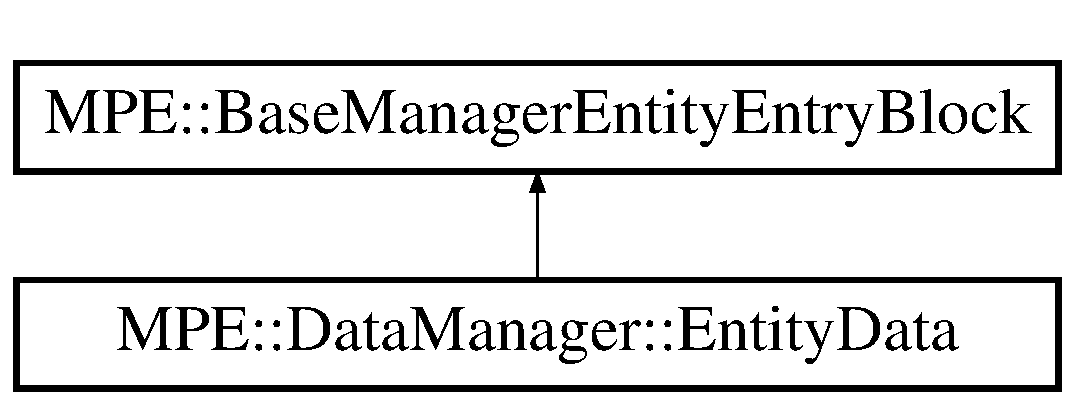
\includegraphics[height=2.000000cm]{struct_m_p_e_1_1_data_manager_1_1_entity_data}
\end{center}
\end{figure}
\subsection*{Public Attributes}
\begin{DoxyCompactItemize}
\item 
\hyperlink{struct_m_p_e_1_1_data_manager_1_1_data_buffer}{Data\+Buffer} $\ast$$\ast$ \hyperlink{struct_m_p_e_1_1_data_manager_1_1_entity_data_a93b9cee26b2194ff28d2d6c659b0fa97}{data\+Buff}
\end{DoxyCompactItemize}


\subsection{Detailed Description}
The managers \hyperlink{struct_m_p_e_1_1_entity}{Entity} entry block. 

\subsection{Member Data Documentation}
\mbox{\Hypertarget{struct_m_p_e_1_1_data_manager_1_1_entity_data_a93b9cee26b2194ff28d2d6c659b0fa97}\label{struct_m_p_e_1_1_data_manager_1_1_entity_data_a93b9cee26b2194ff28d2d6c659b0fa97}} 
\index{M\+P\+E\+::\+Data\+Manager\+::\+Entity\+Data@{M\+P\+E\+::\+Data\+Manager\+::\+Entity\+Data}!data\+Buff@{data\+Buff}}
\index{data\+Buff@{data\+Buff}!M\+P\+E\+::\+Data\+Manager\+::\+Entity\+Data@{M\+P\+E\+::\+Data\+Manager\+::\+Entity\+Data}}
\subsubsection{\texorpdfstring{data\+Buff}{dataBuff}}
{\footnotesize\ttfamily \hyperlink{struct_m_p_e_1_1_data_manager_1_1_data_buffer}{Data\+Buffer}$\ast$$\ast$ M\+P\+E\+::\+Data\+Manager\+::\+Entity\+Data\+::data\+Buff}

Stores a pointer to the data entries for the \hyperlink{struct_m_p_e_1_1_entity}{Entity} entry 

The documentation for this struct was generated from the following file\+:\begin{DoxyCompactItemize}
\item 
\hyperlink{_data_manager_8h}{Data\+Manager.\+h}\end{DoxyCompactItemize}

\hypertarget{struct_m_p_e_1_1_entity_hasher}{}\section{M\+PE\+:\+:Entity\+Hasher Struct Reference}
\label{struct_m_p_e_1_1_entity_hasher}\index{M\+P\+E\+::\+Entity\+Hasher@{M\+P\+E\+::\+Entity\+Hasher}}


{\ttfamily \#include $<$Entity.\+h$>$}

\subsection*{Public Member Functions}
\begin{DoxyCompactItemize}
\item 
size\+\_\+t \hyperlink{struct_m_p_e_1_1_entity_hasher_a31881f56120ff3a108eaa447c7093b96}{operator()} (const \hyperlink{struct_m_p_e_1_1_entity}{Entity} \&key) const
\end{DoxyCompactItemize}


\subsection{Member Function Documentation}
\mbox{\Hypertarget{struct_m_p_e_1_1_entity_hasher_a31881f56120ff3a108eaa447c7093b96}\label{struct_m_p_e_1_1_entity_hasher_a31881f56120ff3a108eaa447c7093b96}} 
\index{M\+P\+E\+::\+Entity\+Hasher@{M\+P\+E\+::\+Entity\+Hasher}!operator()@{operator()}}
\index{operator()@{operator()}!M\+P\+E\+::\+Entity\+Hasher@{M\+P\+E\+::\+Entity\+Hasher}}
\subsubsection{\texorpdfstring{operator()()}{operator()()}}
{\footnotesize\ttfamily size\+\_\+t M\+P\+E\+::\+Entity\+Hasher\+::operator() (\begin{DoxyParamCaption}\item[{const \hyperlink{struct_m_p_e_1_1_entity}{Entity} \&}]{key }\end{DoxyParamCaption}) const\hspace{0.3cm}{\ttfamily [inline]}}



The documentation for this struct was generated from the following file\+:\begin{DoxyCompactItemize}
\item 
\hyperlink{_entity_8h}{Entity.\+h}\end{DoxyCompactItemize}

\hypertarget{struct_m_p_e_1_1_data_manager_1_1_entry_header}{}\section{M\+PE\+:\+:Data\+Manager\+:\+:Entry\+Header Struct Reference}
\label{struct_m_p_e_1_1_data_manager_1_1_entry_header}\index{M\+P\+E\+::\+Data\+Manager\+::\+Entry\+Header@{M\+P\+E\+::\+Data\+Manager\+::\+Entry\+Header}}


The header struct, used for keeping track of the data entries an \hyperlink{struct_m_p_e_1_1_entity}{Entity} has.  


\subsection*{Public Attributes}
\begin{DoxyCompactItemize}
\item 
uint8\+\_\+t \hyperlink{struct_m_p_e_1_1_data_manager_1_1_entry_header_a0d7adc0b636e8c00d1d38b6b780a96da}{capacity} = 0
\item 
uint8\+\_\+t \hyperlink{struct_m_p_e_1_1_data_manager_1_1_entry_header_ae1f8d7e4b6363ba5af82c1c20b7a9d1f}{entry\+Count} = 0
\item 
uint32\+\_\+t $\ast$ \hyperlink{struct_m_p_e_1_1_data_manager_1_1_entry_header_a1147ac0d74ba9de830139b4f661a92c7}{keys}
\item 
\hyperlink{class_m_p_e_1_1_data_manager_aeebd98a9feed805f5ebd63276f003f5f}{Data\+Type} $\ast$ \hyperlink{struct_m_p_e_1_1_data_manager_1_1_entry_header_aff785b6cab9ad54f0f3a14e3f4ca5a11}{type}
\item 
\hyperlink{struct_m_p_e_1_1_data_manager_1_1_value}{Value} $\ast$ \hyperlink{struct_m_p_e_1_1_data_manager_1_1_entry_header_a56c968449fa90b40890ec0f9ec8b3736}{value}
\end{DoxyCompactItemize}
\subsection*{Static Public Attributes}
\begin{DoxyCompactItemize}
\item 
static const uint8\+\_\+t \hyperlink{struct_m_p_e_1_1_data_manager_1_1_entry_header_a8b73487b833524d0b1497e07f5f63129}{entry\+Size} = sizeof(uint32\+\_\+t) + sizeof(\hyperlink{class_m_p_e_1_1_data_manager_aeebd98a9feed805f5ebd63276f003f5f}{Data\+Type}) + sizeof(\hyperlink{struct_m_p_e_1_1_data_manager_1_1_value}{Value})
\end{DoxyCompactItemize}


\subsection{Detailed Description}
The header struct, used for keeping track of the data entries an \hyperlink{struct_m_p_e_1_1_entity}{Entity} has. 

\subsection{Member Data Documentation}
\mbox{\Hypertarget{struct_m_p_e_1_1_data_manager_1_1_entry_header_a0d7adc0b636e8c00d1d38b6b780a96da}\label{struct_m_p_e_1_1_data_manager_1_1_entry_header_a0d7adc0b636e8c00d1d38b6b780a96da}} 
\index{M\+P\+E\+::\+Data\+Manager\+::\+Entry\+Header@{M\+P\+E\+::\+Data\+Manager\+::\+Entry\+Header}!capacity@{capacity}}
\index{capacity@{capacity}!M\+P\+E\+::\+Data\+Manager\+::\+Entry\+Header@{M\+P\+E\+::\+Data\+Manager\+::\+Entry\+Header}}
\subsubsection{\texorpdfstring{capacity}{capacity}}
{\footnotesize\ttfamily uint8\+\_\+t M\+P\+E\+::\+Data\+Manager\+::\+Entry\+Header\+::capacity = 0}

\mbox{\Hypertarget{struct_m_p_e_1_1_data_manager_1_1_entry_header_ae1f8d7e4b6363ba5af82c1c20b7a9d1f}\label{struct_m_p_e_1_1_data_manager_1_1_entry_header_ae1f8d7e4b6363ba5af82c1c20b7a9d1f}} 
\index{M\+P\+E\+::\+Data\+Manager\+::\+Entry\+Header@{M\+P\+E\+::\+Data\+Manager\+::\+Entry\+Header}!entry\+Count@{entry\+Count}}
\index{entry\+Count@{entry\+Count}!M\+P\+E\+::\+Data\+Manager\+::\+Entry\+Header@{M\+P\+E\+::\+Data\+Manager\+::\+Entry\+Header}}
\subsubsection{\texorpdfstring{entry\+Count}{entryCount}}
{\footnotesize\ttfamily uint8\+\_\+t M\+P\+E\+::\+Data\+Manager\+::\+Entry\+Header\+::entry\+Count = 0}

\mbox{\Hypertarget{struct_m_p_e_1_1_data_manager_1_1_entry_header_a8b73487b833524d0b1497e07f5f63129}\label{struct_m_p_e_1_1_data_manager_1_1_entry_header_a8b73487b833524d0b1497e07f5f63129}} 
\index{M\+P\+E\+::\+Data\+Manager\+::\+Entry\+Header@{M\+P\+E\+::\+Data\+Manager\+::\+Entry\+Header}!entry\+Size@{entry\+Size}}
\index{entry\+Size@{entry\+Size}!M\+P\+E\+::\+Data\+Manager\+::\+Entry\+Header@{M\+P\+E\+::\+Data\+Manager\+::\+Entry\+Header}}
\subsubsection{\texorpdfstring{entry\+Size}{entrySize}}
{\footnotesize\ttfamily const uint8\+\_\+t M\+P\+E\+::\+Data\+Manager\+::\+Entry\+Header\+::entry\+Size = sizeof(uint32\+\_\+t) + sizeof(\hyperlink{class_m_p_e_1_1_data_manager_aeebd98a9feed805f5ebd63276f003f5f}{Data\+Type}) + sizeof(\hyperlink{struct_m_p_e_1_1_data_manager_1_1_value}{Value})\hspace{0.3cm}{\ttfamily [static]}}

\mbox{\Hypertarget{struct_m_p_e_1_1_data_manager_1_1_entry_header_a1147ac0d74ba9de830139b4f661a92c7}\label{struct_m_p_e_1_1_data_manager_1_1_entry_header_a1147ac0d74ba9de830139b4f661a92c7}} 
\index{M\+P\+E\+::\+Data\+Manager\+::\+Entry\+Header@{M\+P\+E\+::\+Data\+Manager\+::\+Entry\+Header}!keys@{keys}}
\index{keys@{keys}!M\+P\+E\+::\+Data\+Manager\+::\+Entry\+Header@{M\+P\+E\+::\+Data\+Manager\+::\+Entry\+Header}}
\subsubsection{\texorpdfstring{keys}{keys}}
{\footnotesize\ttfamily uint32\+\_\+t$\ast$ M\+P\+E\+::\+Data\+Manager\+::\+Entry\+Header\+::keys}

\mbox{\Hypertarget{struct_m_p_e_1_1_data_manager_1_1_entry_header_aff785b6cab9ad54f0f3a14e3f4ca5a11}\label{struct_m_p_e_1_1_data_manager_1_1_entry_header_aff785b6cab9ad54f0f3a14e3f4ca5a11}} 
\index{M\+P\+E\+::\+Data\+Manager\+::\+Entry\+Header@{M\+P\+E\+::\+Data\+Manager\+::\+Entry\+Header}!type@{type}}
\index{type@{type}!M\+P\+E\+::\+Data\+Manager\+::\+Entry\+Header@{M\+P\+E\+::\+Data\+Manager\+::\+Entry\+Header}}
\subsubsection{\texorpdfstring{type}{type}}
{\footnotesize\ttfamily \hyperlink{class_m_p_e_1_1_data_manager_aeebd98a9feed805f5ebd63276f003f5f}{Data\+Type}$\ast$ M\+P\+E\+::\+Data\+Manager\+::\+Entry\+Header\+::type}

\mbox{\Hypertarget{struct_m_p_e_1_1_data_manager_1_1_entry_header_a56c968449fa90b40890ec0f9ec8b3736}\label{struct_m_p_e_1_1_data_manager_1_1_entry_header_a56c968449fa90b40890ec0f9ec8b3736}} 
\index{M\+P\+E\+::\+Data\+Manager\+::\+Entry\+Header@{M\+P\+E\+::\+Data\+Manager\+::\+Entry\+Header}!value@{value}}
\index{value@{value}!M\+P\+E\+::\+Data\+Manager\+::\+Entry\+Header@{M\+P\+E\+::\+Data\+Manager\+::\+Entry\+Header}}
\subsubsection{\texorpdfstring{value}{value}}
{\footnotesize\ttfamily \hyperlink{struct_m_p_e_1_1_data_manager_1_1_value}{Value}$\ast$ M\+P\+E\+::\+Data\+Manager\+::\+Entry\+Header\+::value}



The documentation for this struct was generated from the following file\+:\begin{DoxyCompactItemize}
\item 
\hyperlink{_data_manager_8h}{Data\+Manager.\+h}\end{DoxyCompactItemize}

\hypertarget{class_m_p_e_1_1_manager}{}\section{M\+PE\+:\+:Manager Class Reference}
\label{class_m_p_e_1_1_manager}\index{M\+P\+E\+::\+Manager@{M\+P\+E\+::\+Manager}}


The manager base class.  




{\ttfamily \#include $<$Manager.\+h$>$}

Inheritance diagram for M\+PE\+:\+:Manager\+:\begin{figure}[H]
\begin{center}
\leavevmode
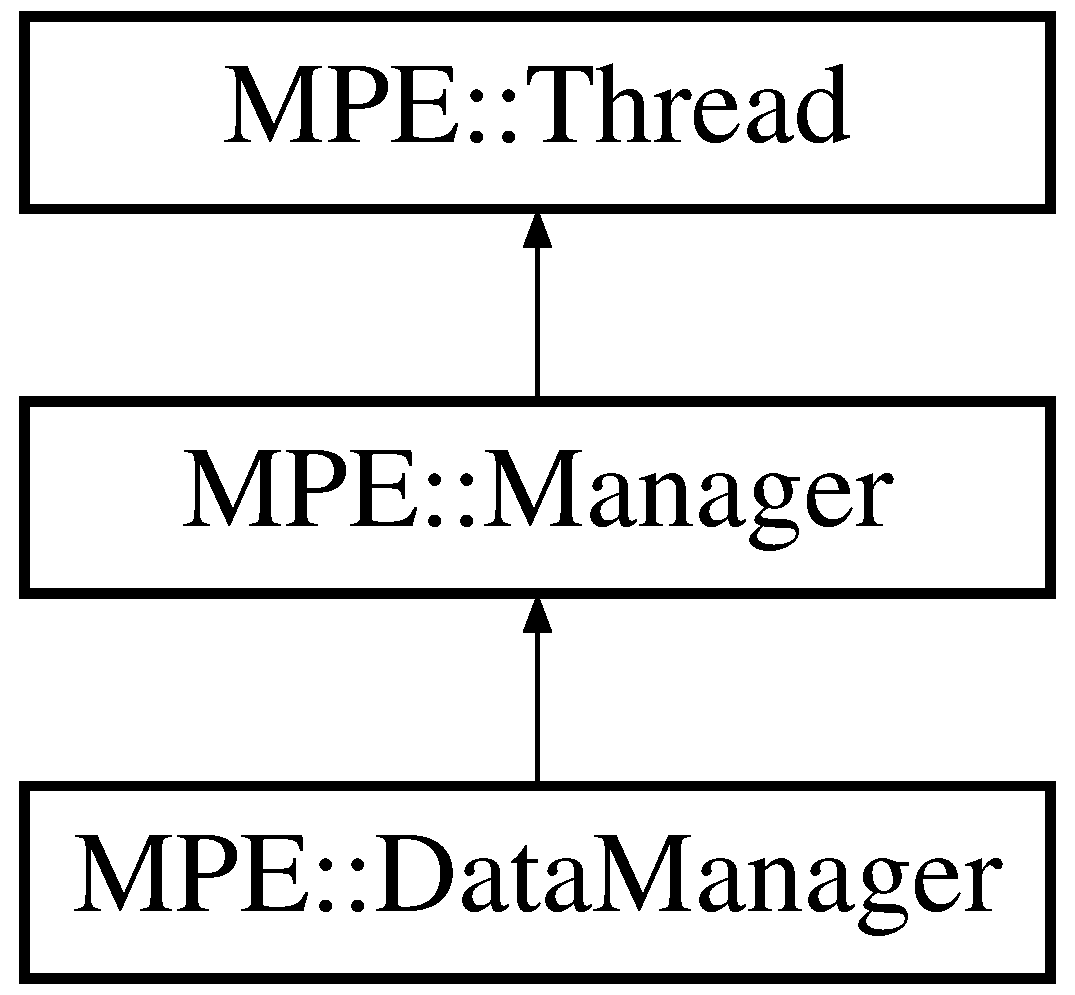
\includegraphics[height=3.000000cm]{class_m_p_e_1_1_manager}
\end{center}
\end{figure}
\subsection*{Protected Member Functions}
\begin{DoxyCompactItemize}
\item 
\hyperlink{class_m_p_e_1_1_manager_a16591d627df08536ce27b7d791347269}{Manager} (\hyperlink{struct_m_p_e_1_1_base_manager_entity_entry_block}{Base\+Manager\+Entity\+Entry\+Block} $\ast$entires, \hyperlink{namespace_m_p_e_a16447295e3105bd2ba2a9ea303566175}{thread\+Identifier} identifier, uint8\+\_\+t frame\+Sync\+Time=16)
\item 
virtual \hyperlink{class_m_p_e_1_1_manager_a6bf168edb75ff564f1dee7a9869798f0}{$\sim$\+Manager} ()
\end{DoxyCompactItemize}
\subsection*{Protected Attributes}
\begin{DoxyCompactItemize}
\item 
std\+::unordered\+\_\+map$<$ \hyperlink{struct_m_p_e_1_1_entity}{Entity}, uint32\+\_\+t, \hyperlink{struct_m_p_e_1_1_entity_hasher}{Entity\+Hasher} $>$ \hyperlink{class_m_p_e_1_1_manager_a142d48cdd0daf0b9ad667ea599de586a}{\+\_\+entity\+To\+Index}
\end{DoxyCompactItemize}
\subsection*{Private Attributes}
\begin{DoxyCompactItemize}
\item 
\hyperlink{struct_m_p_e_1_1_base_manager_entity_entry_block}{Base\+Manager\+Entity\+Entry\+Block} $\ast$ \hyperlink{class_m_p_e_1_1_manager_a5d8d764913aecc8a92ad83790570df86}{\+\_\+base\+Entity\+Entires}
\end{DoxyCompactItemize}
\subsection*{Additional Inherited Members}


\subsection{Detailed Description}
The manager base class. 

This is a virtual class and is intended to be inherited by classes are to be used as component managers for entities. 

\subsection{Constructor \& Destructor Documentation}
\mbox{\Hypertarget{class_m_p_e_1_1_manager_a16591d627df08536ce27b7d791347269}\label{class_m_p_e_1_1_manager_a16591d627df08536ce27b7d791347269}} 
\index{M\+P\+E\+::\+Manager@{M\+P\+E\+::\+Manager}!Manager@{Manager}}
\index{Manager@{Manager}!M\+P\+E\+::\+Manager@{M\+P\+E\+::\+Manager}}
\subsubsection{\texorpdfstring{Manager()}{Manager()}}
{\footnotesize\ttfamily M\+P\+E\+::\+Manager\+::\+Manager (\begin{DoxyParamCaption}\item[{\hyperlink{struct_m_p_e_1_1_base_manager_entity_entry_block}{Base\+Manager\+Entity\+Entry\+Block} $\ast$}]{entires,  }\item[{\hyperlink{namespace_m_p_e_a16447295e3105bd2ba2a9ea303566175}{thread\+Identifier}}]{identifier,  }\item[{uint8\+\_\+t}]{frame\+Sync\+Time = {\ttfamily 16} }\end{DoxyParamCaption})\hspace{0.3cm}{\ttfamily [protected]}}

\mbox{\Hypertarget{class_m_p_e_1_1_manager_a6bf168edb75ff564f1dee7a9869798f0}\label{class_m_p_e_1_1_manager_a6bf168edb75ff564f1dee7a9869798f0}} 
\index{M\+P\+E\+::\+Manager@{M\+P\+E\+::\+Manager}!````~Manager@{$\sim$\+Manager}}
\index{````~Manager@{$\sim$\+Manager}!M\+P\+E\+::\+Manager@{M\+P\+E\+::\+Manager}}
\subsubsection{\texorpdfstring{$\sim$\+Manager()}{~Manager()}}
{\footnotesize\ttfamily M\+P\+E\+::\+Manager\+::$\sim$\+Manager (\begin{DoxyParamCaption}{ }\end{DoxyParamCaption})\hspace{0.3cm}{\ttfamily [protected]}, {\ttfamily [virtual]}}



\subsection{Member Data Documentation}
\mbox{\Hypertarget{class_m_p_e_1_1_manager_a5d8d764913aecc8a92ad83790570df86}\label{class_m_p_e_1_1_manager_a5d8d764913aecc8a92ad83790570df86}} 
\index{M\+P\+E\+::\+Manager@{M\+P\+E\+::\+Manager}!\+\_\+base\+Entity\+Entires@{\+\_\+base\+Entity\+Entires}}
\index{\+\_\+base\+Entity\+Entires@{\+\_\+base\+Entity\+Entires}!M\+P\+E\+::\+Manager@{M\+P\+E\+::\+Manager}}
\subsubsection{\texorpdfstring{\+\_\+base\+Entity\+Entires}{\_baseEntityEntires}}
{\footnotesize\ttfamily \hyperlink{struct_m_p_e_1_1_base_manager_entity_entry_block}{Base\+Manager\+Entity\+Entry\+Block}$\ast$ M\+P\+E\+::\+Manager\+::\+\_\+base\+Entity\+Entires\hspace{0.3cm}{\ttfamily [private]}}

\mbox{\Hypertarget{class_m_p_e_1_1_manager_a142d48cdd0daf0b9ad667ea599de586a}\label{class_m_p_e_1_1_manager_a142d48cdd0daf0b9ad667ea599de586a}} 
\index{M\+P\+E\+::\+Manager@{M\+P\+E\+::\+Manager}!\+\_\+entity\+To\+Index@{\+\_\+entity\+To\+Index}}
\index{\+\_\+entity\+To\+Index@{\+\_\+entity\+To\+Index}!M\+P\+E\+::\+Manager@{M\+P\+E\+::\+Manager}}
\subsubsection{\texorpdfstring{\+\_\+entity\+To\+Index}{\_entityToIndex}}
{\footnotesize\ttfamily std\+::unordered\+\_\+map$<$\hyperlink{struct_m_p_e_1_1_entity}{Entity}, uint32\+\_\+t, \hyperlink{struct_m_p_e_1_1_entity_hasher}{Entity\+Hasher}$>$ M\+P\+E\+::\+Manager\+::\+\_\+entity\+To\+Index\hspace{0.3cm}{\ttfamily [protected]}}



The documentation for this class was generated from the following files\+:\begin{DoxyCompactItemize}
\item 
\hyperlink{_manager_8h}{Manager.\+h}\item 
\hyperlink{_manager_8cpp}{Manager.\+cpp}\end{DoxyCompactItemize}

\hypertarget{struct_m_p_e_1_1_msg}{}\section{M\+PE\+:\+:Msg Struct Reference}
\label{struct_m_p_e_1_1_msg}\index{M\+P\+E\+::\+Msg@{M\+P\+E\+::\+Msg}}


{\ttfamily \#include $<$Msg.\+h$>$}

\subsection*{Public Attributes}
\begin{DoxyCompactItemize}
\item 
void $\ast$ \hyperlink{struct_m_p_e_1_1_msg_afd324f2a137a0ecfffdb3cc46703184f}{data}
\item 
uint32\+\_\+t \hyperlink{struct_m_p_e_1_1_msg_a5fd5790137b7e5916b13c7a5375cc6f3}{src}
\item 
uint32\+\_\+t \hyperlink{struct_m_p_e_1_1_msg_a04b1b5fb0cdbb84226609f15d621e21b}{tag}
\item 
uint8\+\_\+t \hyperlink{struct_m_p_e_1_1_msg_a6866bacef848a944fd3b33f88cfedcc4}{prio}
\end{DoxyCompactItemize}


\subsection{Member Data Documentation}
\mbox{\Hypertarget{struct_m_p_e_1_1_msg_afd324f2a137a0ecfffdb3cc46703184f}\label{struct_m_p_e_1_1_msg_afd324f2a137a0ecfffdb3cc46703184f}} 
\index{M\+P\+E\+::\+Msg@{M\+P\+E\+::\+Msg}!data@{data}}
\index{data@{data}!M\+P\+E\+::\+Msg@{M\+P\+E\+::\+Msg}}
\subsubsection{\texorpdfstring{data}{data}}
{\footnotesize\ttfamily void$\ast$ M\+P\+E\+::\+Msg\+::data}

\mbox{\Hypertarget{struct_m_p_e_1_1_msg_a6866bacef848a944fd3b33f88cfedcc4}\label{struct_m_p_e_1_1_msg_a6866bacef848a944fd3b33f88cfedcc4}} 
\index{M\+P\+E\+::\+Msg@{M\+P\+E\+::\+Msg}!prio@{prio}}
\index{prio@{prio}!M\+P\+E\+::\+Msg@{M\+P\+E\+::\+Msg}}
\subsubsection{\texorpdfstring{prio}{prio}}
{\footnotesize\ttfamily uint8\+\_\+t M\+P\+E\+::\+Msg\+::prio}

\mbox{\Hypertarget{struct_m_p_e_1_1_msg_a5fd5790137b7e5916b13c7a5375cc6f3}\label{struct_m_p_e_1_1_msg_a5fd5790137b7e5916b13c7a5375cc6f3}} 
\index{M\+P\+E\+::\+Msg@{M\+P\+E\+::\+Msg}!src@{src}}
\index{src@{src}!M\+P\+E\+::\+Msg@{M\+P\+E\+::\+Msg}}
\subsubsection{\texorpdfstring{src}{src}}
{\footnotesize\ttfamily uint32\+\_\+t M\+P\+E\+::\+Msg\+::src}

Source, if Msg\+\_\+\+Any\+\_\+\+Src was specified. \mbox{\Hypertarget{struct_m_p_e_1_1_msg_a04b1b5fb0cdbb84226609f15d621e21b}\label{struct_m_p_e_1_1_msg_a04b1b5fb0cdbb84226609f15d621e21b}} 
\index{M\+P\+E\+::\+Msg@{M\+P\+E\+::\+Msg}!tag@{tag}}
\index{tag@{tag}!M\+P\+E\+::\+Msg@{M\+P\+E\+::\+Msg}}
\subsubsection{\texorpdfstring{tag}{tag}}
{\footnotesize\ttfamily uint32\+\_\+t M\+P\+E\+::\+Msg\+::tag}

\hyperlink{namespace_m_p_e_1_1_tag}{Tag}, if \hyperlink{namespace_m_p_e_1_1_tag_aa5b0456e2af78c51452dd5a5a9b39b8c}{Tag\+::\+Any} was specified. 

The documentation for this struct was generated from the following file\+:\begin{DoxyCompactItemize}
\item 
\hyperlink{_msg_8h}{Msg.\+h}\end{DoxyCompactItemize}

\hypertarget{struct_m_p_e_1_1_msg_comp}{}\section{M\+PE\+:\+:Msg\+Comp Struct Reference}
\label{struct_m_p_e_1_1_msg_comp}\index{M\+P\+E\+::\+Msg\+Comp@{M\+P\+E\+::\+Msg\+Comp}}


{\ttfamily \#include $<$Msg.\+h$>$}

\subsection*{Public Member Functions}
\begin{DoxyCompactItemize}
\item 
bool \hyperlink{struct_m_p_e_1_1_msg_comp_ac56d9edd535cc84e7ea1b918d06c8ecd}{operator()} (const \hyperlink{struct_m_p_e_1_1_msg}{Msg} \&lhs, const \hyperlink{struct_m_p_e_1_1_msg}{Msg} \&rhs) const
\end{DoxyCompactItemize}


\subsection{Member Function Documentation}
\mbox{\Hypertarget{struct_m_p_e_1_1_msg_comp_ac56d9edd535cc84e7ea1b918d06c8ecd}\label{struct_m_p_e_1_1_msg_comp_ac56d9edd535cc84e7ea1b918d06c8ecd}} 
\index{M\+P\+E\+::\+Msg\+Comp@{M\+P\+E\+::\+Msg\+Comp}!operator()@{operator()}}
\index{operator()@{operator()}!M\+P\+E\+::\+Msg\+Comp@{M\+P\+E\+::\+Msg\+Comp}}
\subsubsection{\texorpdfstring{operator()()}{operator()()}}
{\footnotesize\ttfamily bool M\+P\+E\+::\+Msg\+Comp\+::operator() (\begin{DoxyParamCaption}\item[{const \hyperlink{struct_m_p_e_1_1_msg}{Msg} \&}]{lhs,  }\item[{const \hyperlink{struct_m_p_e_1_1_msg}{Msg} \&}]{rhs }\end{DoxyParamCaption}) const\hspace{0.3cm}{\ttfamily [inline]}}



The documentation for this struct was generated from the following file\+:\begin{DoxyCompactItemize}
\item 
\hyperlink{_msg_8h}{Msg.\+h}\end{DoxyCompactItemize}

\hypertarget{class_profiler}{}\section{Profiler Class Reference}
\label{class_profiler}\index{Profiler@{Profiler}}


{\ttfamily \#include $<$Profiler.\+h$>$}

\subsection*{Classes}
\begin{DoxyCompactItemize}
\item 
struct \hyperlink{struct_profiler_1_1_data}{Data}
\end{DoxyCompactItemize}
\subsection*{Public Member Functions}
\begin{DoxyCompactItemize}
\item 
{\footnotesize template$<$uint64\+\_\+t function\+Hash$>$ }\\const void \hyperlink{class_profiler_a1d9623c49b247e4b8374dd991d489f45}{Start\+ProfileF} (const char $\ast$func\+Name)
\item 
const void \hyperlink{class_profiler_a6f9e7815c9d08f33ec89f3aedbb85694}{Stop\+ProfileF} (uint32\+\_\+t threadid)
\item 
const void \hyperlink{class_profiler_af6216cfe94749776e49a0886fa91b96c}{\+\_\+dump\+To\+File} ()
\end{DoxyCompactItemize}
\subsection*{Static Public Member Functions}
\begin{DoxyCompactItemize}
\item 
static \hyperlink{class_profiler}{Profiler} \& \hyperlink{class_profiler_af260850db5b9767c969973090c845ab4}{Get\+Instance} ()
\end{DoxyCompactItemize}
\subsection*{Private Member Functions}
\begin{DoxyCompactItemize}
\item 
\hyperlink{class_profiler_a675ebc9207b9aeace1d967c085abeacf}{Profiler} ()
\item 
\hyperlink{class_profiler_a1e6dd8f6cfb15cd5237b971d8f49c749}{$\sim$\+Profiler} ()
\end{DoxyCompactItemize}
\subsection*{Private Attributes}
\begin{DoxyCompactItemize}
\item 
\hyperlink{struct_profiler_1_1_data}{Data} $\ast$ \hyperlink{class_profiler_a862fb21ca07c94f5f657c7cd1a053a33}{\+\_\+profile} = nullptr
\item 
\hyperlink{struct_profiler_1_1_data}{Data} $\ast$ \hyperlink{class_profiler_a2d8b680e39756a8451e49ae51696d010}{\+\_\+current} = nullptr
\end{DoxyCompactItemize}


\subsection{Constructor \& Destructor Documentation}
\mbox{\Hypertarget{class_profiler_a675ebc9207b9aeace1d967c085abeacf}\label{class_profiler_a675ebc9207b9aeace1d967c085abeacf}} 
\index{Profiler@{Profiler}!Profiler@{Profiler}}
\index{Profiler@{Profiler}!Profiler@{Profiler}}
\subsubsection{\texorpdfstring{Profiler()}{Profiler()}}
{\footnotesize\ttfamily Profiler\+::\+Profiler (\begin{DoxyParamCaption}{ }\end{DoxyParamCaption})\hspace{0.3cm}{\ttfamily [private]}}

\mbox{\Hypertarget{class_profiler_a1e6dd8f6cfb15cd5237b971d8f49c749}\label{class_profiler_a1e6dd8f6cfb15cd5237b971d8f49c749}} 
\index{Profiler@{Profiler}!````~Profiler@{$\sim$\+Profiler}}
\index{````~Profiler@{$\sim$\+Profiler}!Profiler@{Profiler}}
\subsubsection{\texorpdfstring{$\sim$\+Profiler()}{~Profiler()}}
{\footnotesize\ttfamily Profiler\+::$\sim$\+Profiler (\begin{DoxyParamCaption}{ }\end{DoxyParamCaption})\hspace{0.3cm}{\ttfamily [private]}}



\subsection{Member Function Documentation}
\mbox{\Hypertarget{class_profiler_af6216cfe94749776e49a0886fa91b96c}\label{class_profiler_af6216cfe94749776e49a0886fa91b96c}} 
\index{Profiler@{Profiler}!\+\_\+dump\+To\+File@{\+\_\+dump\+To\+File}}
\index{\+\_\+dump\+To\+File@{\+\_\+dump\+To\+File}!Profiler@{Profiler}}
\subsubsection{\texorpdfstring{\+\_\+dump\+To\+File()}{\_dumpToFile()}}
{\footnotesize\ttfamily const void Profiler\+::\+\_\+dump\+To\+File (\begin{DoxyParamCaption}{ }\end{DoxyParamCaption})}

\mbox{\Hypertarget{class_profiler_af260850db5b9767c969973090c845ab4}\label{class_profiler_af260850db5b9767c969973090c845ab4}} 
\index{Profiler@{Profiler}!Get\+Instance@{Get\+Instance}}
\index{Get\+Instance@{Get\+Instance}!Profiler@{Profiler}}
\subsubsection{\texorpdfstring{Get\+Instance()}{GetInstance()}}
{\footnotesize\ttfamily static \hyperlink{class_profiler}{Profiler}\& Profiler\+::\+Get\+Instance (\begin{DoxyParamCaption}{ }\end{DoxyParamCaption})\hspace{0.3cm}{\ttfamily [static]}}

\mbox{\Hypertarget{class_profiler_a1d9623c49b247e4b8374dd991d489f45}\label{class_profiler_a1d9623c49b247e4b8374dd991d489f45}} 
\index{Profiler@{Profiler}!Start\+ProfileF@{Start\+ProfileF}}
\index{Start\+ProfileF@{Start\+ProfileF}!Profiler@{Profiler}}
\subsubsection{\texorpdfstring{Start\+Profile\+F()}{StartProfileF()}}
{\footnotesize\ttfamily template$<$uint64\+\_\+t function\+Hash$>$ \\
const void Profiler\+::\+Start\+ProfileF (\begin{DoxyParamCaption}\item[{const char $\ast$}]{func\+Name }\end{DoxyParamCaption})\hspace{0.3cm}{\ttfamily [inline]}}

\mbox{\Hypertarget{class_profiler_a6f9e7815c9d08f33ec89f3aedbb85694}\label{class_profiler_a6f9e7815c9d08f33ec89f3aedbb85694}} 
\index{Profiler@{Profiler}!Stop\+ProfileF@{Stop\+ProfileF}}
\index{Stop\+ProfileF@{Stop\+ProfileF}!Profiler@{Profiler}}
\subsubsection{\texorpdfstring{Stop\+Profile\+F()}{StopProfileF()}}
{\footnotesize\ttfamily const void Profiler\+::\+Stop\+ProfileF (\begin{DoxyParamCaption}\item[{uint32\+\_\+t}]{threadid }\end{DoxyParamCaption})}



\subsection{Member Data Documentation}
\mbox{\Hypertarget{class_profiler_a2d8b680e39756a8451e49ae51696d010}\label{class_profiler_a2d8b680e39756a8451e49ae51696d010}} 
\index{Profiler@{Profiler}!\+\_\+current@{\+\_\+current}}
\index{\+\_\+current@{\+\_\+current}!Profiler@{Profiler}}
\subsubsection{\texorpdfstring{\+\_\+current}{\_current}}
{\footnotesize\ttfamily \hyperlink{struct_profiler_1_1_data}{Data}$\ast$ Profiler\+::\+\_\+current = nullptr\hspace{0.3cm}{\ttfamily [private]}}

\mbox{\Hypertarget{class_profiler_a862fb21ca07c94f5f657c7cd1a053a33}\label{class_profiler_a862fb21ca07c94f5f657c7cd1a053a33}} 
\index{Profiler@{Profiler}!\+\_\+profile@{\+\_\+profile}}
\index{\+\_\+profile@{\+\_\+profile}!Profiler@{Profiler}}
\subsubsection{\texorpdfstring{\+\_\+profile}{\_profile}}
{\footnotesize\ttfamily \hyperlink{struct_profiler_1_1_data}{Data}$\ast$ Profiler\+::\+\_\+profile = nullptr\hspace{0.3cm}{\ttfamily [private]}}



The documentation for this class was generated from the following file\+:\begin{DoxyCompactItemize}
\item 
\hyperlink{_profiler_8h}{Profiler.\+h}\end{DoxyCompactItemize}

\hypertarget{class_m_p_e_1_1_thread}{}\section{M\+PE\+:\+:Thread Class Reference}
\label{class_m_p_e_1_1_thread}\index{M\+P\+E\+::\+Thread@{M\+P\+E\+::\+Thread}}


The thread base class.  




{\ttfamily \#include $<$Thread.\+h$>$}

Inheritance diagram for M\+PE\+:\+:Thread\+:\begin{figure}[H]
\begin{center}
\leavevmode
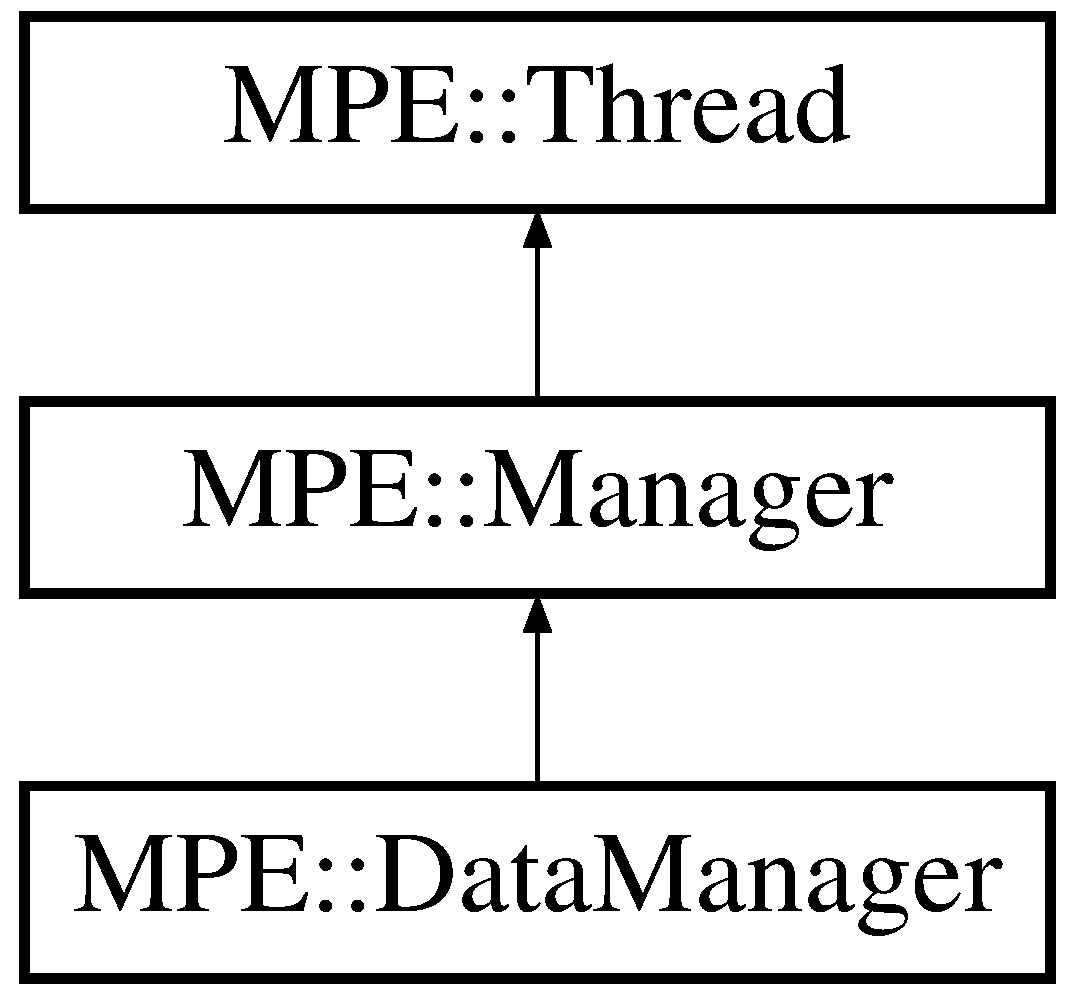
\includegraphics[height=3.000000cm]{class_m_p_e_1_1_thread}
\end{center}
\end{figure}
\subsection*{Public Member Functions}
\begin{DoxyCompactItemize}
\item 
virtual const void \hyperlink{class_m_p_e_1_1_thread_a1bd133a96ec27c868b6bb758e11c0691}{Start} ()=0
\begin{DoxyCompactList}\small\item\em The main entry point for the thread. \end{DoxyCompactList}\item 
\hyperlink{namespace_m_p_e_a16447295e3105bd2ba2a9ea303566175}{thread\+Identifier} \hyperlink{class_m_p_e_1_1_thread_a736d2fc9d527a96419b428e018d225b3}{Get\+Identity} () const
\item 
const void \hyperlink{class_m_p_e_1_1_thread_a1e2ab6a736581d343719f0bba51aa9ad}{Send} (void $\ast$data, uint32\+\_\+t src, uint32\+\_\+t tag, uint8\+\_\+t prio)
\begin{DoxyCompactList}\small\item\em Recvieves message from other thread. \end{DoxyCompactList}\end{DoxyCompactItemize}
\subsection*{Protected Member Functions}
\begin{DoxyCompactItemize}
\item 
\hyperlink{class_m_p_e_1_1_thread_a6b7b08a261115586ae914a9a2325c299}{Thread} (\hyperlink{namespace_m_p_e_a16447295e3105bd2ba2a9ea303566175}{thread\+Identifier} identifier, uint8\+\_\+t frame\+Sync\+Time=16)
\begin{DoxyCompactList}\small\item\em \hyperlink{class_m_p_e_1_1_thread}{Thread} contructor. \end{DoxyCompactList}\item 
virtual \hyperlink{class_m_p_e_1_1_thread_a5addf4f2209106f58447e2c46087c8d7}{$\sim$\+Thread} ()
\item 
const void \hyperlink{class_m_p_e_1_1_thread_a33de6f9fb89f4ae2adf393e866e198da}{Recv} (\hyperlink{struct_m_p_e_1_1_msg}{Msg} \&msg, uint32\+\_\+t src, uint32\+\_\+t tag)
\begin{DoxyCompactList}\small\item\em Recvieve a message. \end{DoxyCompactList}\item 
const uint32\+\_\+t \hyperlink{class_m_p_e_1_1_thread_afa51801ad970ca768ec5160d7c0d7d42}{Peek\+Msg} (\hyperlink{struct_m_p_e_1_1_msg}{Msg} \&msg, uint32\+\_\+t src, uint32\+\_\+t tag)
\begin{DoxyCompactList}\small\item\em Peek message queue. \end{DoxyCompactList}\end{DoxyCompactItemize}
\subsection*{Protected Attributes}
\begin{DoxyCompactItemize}
\item 
\hyperlink{namespace_m_p_e_a16447295e3105bd2ba2a9ea303566175}{thread\+Identifier} \hyperlink{class_m_p_e_1_1_thread_ab7e98443f40fcf9182ea7bf954b8aaf2}{\+\_\+identity}
\item 
uint8\+\_\+t \hyperlink{class_m_p_e_1_1_thread_ad004c47c4002461c874eae460e18ed2a}{\+\_\+frame\+Sync\+Time}
\item 
std\+::priority\+\_\+queue$<$ \hyperlink{struct_m_p_e_1_1_msg}{Msg}, std\+::vector$<$ \hyperlink{struct_m_p_e_1_1_msg}{Msg} $>$, \hyperlink{struct_m_p_e_1_1_msg_comp}{Msg\+Comp} $>$ \hyperlink{class_m_p_e_1_1_thread_a1484f887be46d595bd49c84eef9911ee}{\+\_\+message\+Queue}
\end{DoxyCompactItemize}
\subsection*{Private Attributes}
\begin{DoxyCompactItemize}
\item 
std\+::mutex \hyperlink{class_m_p_e_1_1_thread_af03852c385981359d28bf776370aae3a}{\+\_\+write\+Lock}
\end{DoxyCompactItemize}


\subsection{Detailed Description}
The thread base class. 

This is a virtual class and is intended to be inherited by classes that wishes to use the \hyperlink{class_m_p_e_1_1_thread_message_controller}{Thread\+Message\+Controller}. \begin{DoxySeeAlso}{See also}
\hyperlink{class_m_p_e_1_1_thread_message_controller}{Thread\+Message\+Controller} 
\end{DoxySeeAlso}


\subsection{Constructor \& Destructor Documentation}
\mbox{\Hypertarget{class_m_p_e_1_1_thread_a6b7b08a261115586ae914a9a2325c299}\label{class_m_p_e_1_1_thread_a6b7b08a261115586ae914a9a2325c299}} 
\index{M\+P\+E\+::\+Thread@{M\+P\+E\+::\+Thread}!Thread@{Thread}}
\index{Thread@{Thread}!M\+P\+E\+::\+Thread@{M\+P\+E\+::\+Thread}}
\subsubsection{\texorpdfstring{Thread()}{Thread()}}
{\footnotesize\ttfamily M\+P\+E\+::\+Thread\+::\+Thread (\begin{DoxyParamCaption}\item[{\hyperlink{namespace_m_p_e_a16447295e3105bd2ba2a9ea303566175}{thread\+Identifier}}]{identifier,  }\item[{uint8\+\_\+t}]{frame\+Sync\+Time = {\ttfamily 16} }\end{DoxyParamCaption})\hspace{0.3cm}{\ttfamily [protected]}}



\hyperlink{class_m_p_e_1_1_thread}{Thread} contructor. 


\begin{DoxyParams}{Parameters}
{\em frame\+Sync\+Time} & Limit the thread\textquotesingle{}s frametime to a specific time in ms. \\
\hline
\end{DoxyParams}
\mbox{\Hypertarget{class_m_p_e_1_1_thread_a5addf4f2209106f58447e2c46087c8d7}\label{class_m_p_e_1_1_thread_a5addf4f2209106f58447e2c46087c8d7}} 
\index{M\+P\+E\+::\+Thread@{M\+P\+E\+::\+Thread}!````~Thread@{$\sim$\+Thread}}
\index{````~Thread@{$\sim$\+Thread}!M\+P\+E\+::\+Thread@{M\+P\+E\+::\+Thread}}
\subsubsection{\texorpdfstring{$\sim$\+Thread()}{~Thread()}}
{\footnotesize\ttfamily M\+P\+E\+::\+Thread\+::$\sim$\+Thread (\begin{DoxyParamCaption}{ }\end{DoxyParamCaption})\hspace{0.3cm}{\ttfamily [protected]}, {\ttfamily [virtual]}}



\subsection{Member Function Documentation}
\mbox{\Hypertarget{class_m_p_e_1_1_thread_a736d2fc9d527a96419b428e018d225b3}\label{class_m_p_e_1_1_thread_a736d2fc9d527a96419b428e018d225b3}} 
\index{M\+P\+E\+::\+Thread@{M\+P\+E\+::\+Thread}!Get\+Identity@{Get\+Identity}}
\index{Get\+Identity@{Get\+Identity}!M\+P\+E\+::\+Thread@{M\+P\+E\+::\+Thread}}
\subsubsection{\texorpdfstring{Get\+Identity()}{GetIdentity()}}
{\footnotesize\ttfamily \hyperlink{namespace_m_p_e_a16447295e3105bd2ba2a9ea303566175}{thread\+Identifier} M\+P\+E\+::\+Thread\+::\+Get\+Identity (\begin{DoxyParamCaption}{ }\end{DoxyParamCaption}) const\hspace{0.3cm}{\ttfamily [inline]}}

\mbox{\Hypertarget{class_m_p_e_1_1_thread_afa51801ad970ca768ec5160d7c0d7d42}\label{class_m_p_e_1_1_thread_afa51801ad970ca768ec5160d7c0d7d42}} 
\index{M\+P\+E\+::\+Thread@{M\+P\+E\+::\+Thread}!Peek\+Msg@{Peek\+Msg}}
\index{Peek\+Msg@{Peek\+Msg}!M\+P\+E\+::\+Thread@{M\+P\+E\+::\+Thread}}
\subsubsection{\texorpdfstring{Peek\+Msg()}{PeekMsg()}}
{\footnotesize\ttfamily const uint32\+\_\+t M\+P\+E\+::\+Thread\+::\+Peek\+Msg (\begin{DoxyParamCaption}\item[{\hyperlink{struct_m_p_e_1_1_msg}{Msg} \&}]{msg,  }\item[{uint32\+\_\+t}]{src,  }\item[{uint32\+\_\+t}]{tag }\end{DoxyParamCaption})\hspace{0.3cm}{\ttfamily [protected]}}



Peek message queue. 

This is a non-\/blocking command \begin{DoxySeeAlso}{See also}
\hyperlink{struct_m_p_e_1_1_msg}{Msg} 
\end{DoxySeeAlso}

\begin{DoxyParams}{Parameters}
{\em Src} & Intended destination. Specify \hyperlink{namespace_m_p_e_a0a698f47d1ab10c44a414685c36494f1}{M\+P\+E\+::\+Msg\+\_\+\+Any\+\_\+\+Src} to accept message from any source \\
\hline
{\em tag} & An identifier for the recviever, tags are found in \hyperlink{namespace_m_p_e_1_1_tag}{M\+P\+E\+::\+Tag}, or any user defined tags \\
\hline
\end{DoxyParams}
\begin{DoxyReturn}{Returns}
Returns 0 if no messages in queue, non-\/zero otherwise. 
\end{DoxyReturn}
\begin{DoxySeeAlso}{See also}
\hyperlink{namespace_m_p_e_1_1_tag}{Tag} 
\end{DoxySeeAlso}
\mbox{\Hypertarget{class_m_p_e_1_1_thread_a33de6f9fb89f4ae2adf393e866e198da}\label{class_m_p_e_1_1_thread_a33de6f9fb89f4ae2adf393e866e198da}} 
\index{M\+P\+E\+::\+Thread@{M\+P\+E\+::\+Thread}!Recv@{Recv}}
\index{Recv@{Recv}!M\+P\+E\+::\+Thread@{M\+P\+E\+::\+Thread}}
\subsubsection{\texorpdfstring{Recv()}{Recv()}}
{\footnotesize\ttfamily const void M\+P\+E\+::\+Thread\+::\+Recv (\begin{DoxyParamCaption}\item[{\hyperlink{struct_m_p_e_1_1_msg}{Msg} \&}]{msg,  }\item[{uint32\+\_\+t}]{src,  }\item[{uint32\+\_\+t}]{tag }\end{DoxyParamCaption})\hspace{0.3cm}{\ttfamily [protected]}}



Recvieve a message. 

This is a blocking command. Waits for a specific message. \begin{DoxySeeAlso}{See also}
\hyperlink{struct_m_p_e_1_1_msg}{Msg} 
\end{DoxySeeAlso}

\begin{DoxyParams}{Parameters}
{\em Src} & Intended src. Specify \hyperlink{namespace_m_p_e_a0a698f47d1ab10c44a414685c36494f1}{M\+P\+E\+::\+Msg\+\_\+\+Any\+\_\+\+Src} to accept message from any source \\
\hline
{\em tag} & An identifier for the recviever. \\
\hline
\end{DoxyParams}
\begin{DoxySeeAlso}{See also}
\hyperlink{namespace_m_p_e_1_1_tag}{Tag} 
\end{DoxySeeAlso}
\mbox{\Hypertarget{class_m_p_e_1_1_thread_a1e2ab6a736581d343719f0bba51aa9ad}\label{class_m_p_e_1_1_thread_a1e2ab6a736581d343719f0bba51aa9ad}} 
\index{M\+P\+E\+::\+Thread@{M\+P\+E\+::\+Thread}!Send@{Send}}
\index{Send@{Send}!M\+P\+E\+::\+Thread@{M\+P\+E\+::\+Thread}}
\subsubsection{\texorpdfstring{Send()}{Send()}}
{\footnotesize\ttfamily const void M\+P\+E\+::\+Thread\+::\+Send (\begin{DoxyParamCaption}\item[{void $\ast$}]{data,  }\item[{uint32\+\_\+t}]{src,  }\item[{uint32\+\_\+t}]{tag,  }\item[{uint8\+\_\+t}]{prio }\end{DoxyParamCaption})}



Recvieves message from other thread. 

This is a non-\/blocking command, will continue without wait for message to be delivered. This is called by other threads, not itself. For sending messages see \hyperlink{class_m_p_e_1_1_thread_message_controller_afcc8f572cd1355df9e6a0ef8e2d0f710}{Thread\+Message\+Controller\+::\+Send}. 
\begin{DoxyParams}{Parameters}
{\em data} & Data to be sent \\
\hline
{\em src} & Source \\
\hline
{\em tag} & An identifier for the recviever. \\
\hline
{\em prio} & Priority of the message, 0 is lowest. \\
\hline
\end{DoxyParams}
\begin{DoxySeeAlso}{See also}
\hyperlink{namespace_m_p_e_1_1_tag}{Tag} 
\end{DoxySeeAlso}
\mbox{\Hypertarget{class_m_p_e_1_1_thread_a1bd133a96ec27c868b6bb758e11c0691}\label{class_m_p_e_1_1_thread_a1bd133a96ec27c868b6bb758e11c0691}} 
\index{M\+P\+E\+::\+Thread@{M\+P\+E\+::\+Thread}!Start@{Start}}
\index{Start@{Start}!M\+P\+E\+::\+Thread@{M\+P\+E\+::\+Thread}}
\subsubsection{\texorpdfstring{Start()}{Start()}}
{\footnotesize\ttfamily virtual const void M\+P\+E\+::\+Thread\+::\+Start (\begin{DoxyParamCaption}{ }\end{DoxyParamCaption})\hspace{0.3cm}{\ttfamily [pure virtual]}}



The main entry point for the thread. 



Implemented in \hyperlink{class_m_p_e_1_1_data_manager_aa8d6f1ef687afb532d968a3c1a42f324}{M\+P\+E\+::\+Data\+Manager}.



\subsection{Member Data Documentation}
\mbox{\Hypertarget{class_m_p_e_1_1_thread_ad004c47c4002461c874eae460e18ed2a}\label{class_m_p_e_1_1_thread_ad004c47c4002461c874eae460e18ed2a}} 
\index{M\+P\+E\+::\+Thread@{M\+P\+E\+::\+Thread}!\+\_\+frame\+Sync\+Time@{\+\_\+frame\+Sync\+Time}}
\index{\+\_\+frame\+Sync\+Time@{\+\_\+frame\+Sync\+Time}!M\+P\+E\+::\+Thread@{M\+P\+E\+::\+Thread}}
\subsubsection{\texorpdfstring{\+\_\+frame\+Sync\+Time}{\_frameSyncTime}}
{\footnotesize\ttfamily uint8\+\_\+t M\+P\+E\+::\+Thread\+::\+\_\+frame\+Sync\+Time\hspace{0.3cm}{\ttfamily [protected]}}

\mbox{\Hypertarget{class_m_p_e_1_1_thread_ab7e98443f40fcf9182ea7bf954b8aaf2}\label{class_m_p_e_1_1_thread_ab7e98443f40fcf9182ea7bf954b8aaf2}} 
\index{M\+P\+E\+::\+Thread@{M\+P\+E\+::\+Thread}!\+\_\+identity@{\+\_\+identity}}
\index{\+\_\+identity@{\+\_\+identity}!M\+P\+E\+::\+Thread@{M\+P\+E\+::\+Thread}}
\subsubsection{\texorpdfstring{\+\_\+identity}{\_identity}}
{\footnotesize\ttfamily \hyperlink{namespace_m_p_e_a16447295e3105bd2ba2a9ea303566175}{thread\+Identifier} M\+P\+E\+::\+Thread\+::\+\_\+identity\hspace{0.3cm}{\ttfamily [protected]}}

\mbox{\Hypertarget{class_m_p_e_1_1_thread_a1484f887be46d595bd49c84eef9911ee}\label{class_m_p_e_1_1_thread_a1484f887be46d595bd49c84eef9911ee}} 
\index{M\+P\+E\+::\+Thread@{M\+P\+E\+::\+Thread}!\+\_\+message\+Queue@{\+\_\+message\+Queue}}
\index{\+\_\+message\+Queue@{\+\_\+message\+Queue}!M\+P\+E\+::\+Thread@{M\+P\+E\+::\+Thread}}
\subsubsection{\texorpdfstring{\+\_\+message\+Queue}{\_messageQueue}}
{\footnotesize\ttfamily std\+::priority\+\_\+queue$<$\hyperlink{struct_m_p_e_1_1_msg}{Msg}, std\+::vector$<$\hyperlink{struct_m_p_e_1_1_msg}{Msg}$>$, \hyperlink{struct_m_p_e_1_1_msg_comp}{Msg\+Comp}$>$ M\+P\+E\+::\+Thread\+::\+\_\+message\+Queue\hspace{0.3cm}{\ttfamily [protected]}}

\mbox{\Hypertarget{class_m_p_e_1_1_thread_af03852c385981359d28bf776370aae3a}\label{class_m_p_e_1_1_thread_af03852c385981359d28bf776370aae3a}} 
\index{M\+P\+E\+::\+Thread@{M\+P\+E\+::\+Thread}!\+\_\+write\+Lock@{\+\_\+write\+Lock}}
\index{\+\_\+write\+Lock@{\+\_\+write\+Lock}!M\+P\+E\+::\+Thread@{M\+P\+E\+::\+Thread}}
\subsubsection{\texorpdfstring{\+\_\+write\+Lock}{\_writeLock}}
{\footnotesize\ttfamily std\+::mutex M\+P\+E\+::\+Thread\+::\+\_\+write\+Lock\hspace{0.3cm}{\ttfamily [private]}}



The documentation for this class was generated from the following files\+:\begin{DoxyCompactItemize}
\item 
\hyperlink{_thread_8h}{Thread.\+h}\item 
\hyperlink{_thread_8cpp}{Thread.\+cpp}\end{DoxyCompactItemize}

\hypertarget{class_m_p_e_1_1_thread_message_controller}{}\section{M\+PE\+:\+:Thread\+Message\+Controller Class Reference}
\label{class_m_p_e_1_1_thread_message_controller}\index{M\+P\+E\+::\+Thread\+Message\+Controller@{M\+P\+E\+::\+Thread\+Message\+Controller}}


The \hyperlink{class_m_p_e_1_1_thread_message_controller}{Thread\+Message\+Controller} initiates threads and handles the communication between them.  




{\ttfamily \#include $<$Thread\+Message\+Controller.\+h$>$}

\subsection*{Public Member Functions}
\begin{DoxyCompactItemize}
\item 
const void \hyperlink{class_m_p_e_1_1_thread_message_controller_a08663e963b8ac560e0678527a6f0cd86}{Start\+Thread} (\hyperlink{class_m_p_e_1_1_thread}{Thread} $\ast$thread, double frame\+Sync\+Time)
\begin{DoxyCompactList}\small\item\em Starts a new thread. \end{DoxyCompactList}\item 
const void \hyperlink{class_m_p_e_1_1_thread_message_controller_ad4fdb8a09a50306d1002fd3fb5bae5e3}{Send} (void $\ast$data, size\+\_\+t size, uint32\+\_\+t dest, uint32\+\_\+t tag)
\begin{DoxyCompactList}\small\item\em Send a message. \end{DoxyCompactList}\item 
const void \hyperlink{class_m_p_e_1_1_thread_message_controller_a76ce2d05dfedd82e6d522151d42880f6}{BroadC} (void $\ast$data, size\+\_\+t, uint32\+\_\+t tag)
\begin{DoxyCompactList}\small\item\em Send a Broadcast to all threads. \end{DoxyCompactList}\item 
const void \hyperlink{class_m_p_e_1_1_thread_message_controller_ab55fff1fb40f1456efb7e029fa1ddb89}{Recv} (void $\ast$$\ast$data, size\+\_\+t \&size, uint32\+\_\+t src, uint32\+\_\+t tag)
\begin{DoxyCompactList}\small\item\em Recvieve a message. \end{DoxyCompactList}\item 
const uint32\+\_\+t \hyperlink{class_m_p_e_1_1_thread_message_controller_abfa4aaad59117d2b4f83cf7504d55cb7}{Peek\+Msg} (void $\ast$$\ast$data, size\+\_\+t \&size, uint32\+\_\+t src, uint32\+\_\+t tag)
\begin{DoxyCompactList}\small\item\em Peek message queue. \end{DoxyCompactList}\end{DoxyCompactItemize}


\subsection{Detailed Description}
The \hyperlink{class_m_p_e_1_1_thread_message_controller}{Thread\+Message\+Controller} initiates threads and handles the communication between them. 

\subsection{Member Function Documentation}
\mbox{\Hypertarget{class_m_p_e_1_1_thread_message_controller_a76ce2d05dfedd82e6d522151d42880f6}\label{class_m_p_e_1_1_thread_message_controller_a76ce2d05dfedd82e6d522151d42880f6}} 
\index{M\+P\+E\+::\+Thread\+Message\+Controller@{M\+P\+E\+::\+Thread\+Message\+Controller}!BroadC@{BroadC}}
\index{BroadC@{BroadC}!M\+P\+E\+::\+Thread\+Message\+Controller@{M\+P\+E\+::\+Thread\+Message\+Controller}}
\subsubsection{\texorpdfstring{Broad\+C()}{BroadC()}}
{\footnotesize\ttfamily const void M\+P\+E\+::\+Thread\+Message\+Controller\+::\+BroadC (\begin{DoxyParamCaption}\item[{void $\ast$}]{data,  }\item[{size\+\_\+t}]{,  }\item[{uint32\+\_\+t}]{tag }\end{DoxyParamCaption})}



Send a Broadcast to all threads. 

This is a non-\/blocking command 
\begin{DoxyParams}{Parameters}
{\em data} & Data to be sent \\
\hline
{\em size} & size of data \\
\hline
{\em tag} & An identifier for the recviever. \\
\hline
\end{DoxyParams}
\begin{DoxySeeAlso}{See also}
\hyperlink{struct_tag}{Tag} 
\end{DoxySeeAlso}
\mbox{\Hypertarget{class_m_p_e_1_1_thread_message_controller_abfa4aaad59117d2b4f83cf7504d55cb7}\label{class_m_p_e_1_1_thread_message_controller_abfa4aaad59117d2b4f83cf7504d55cb7}} 
\index{M\+P\+E\+::\+Thread\+Message\+Controller@{M\+P\+E\+::\+Thread\+Message\+Controller}!Peek\+Msg@{Peek\+Msg}}
\index{Peek\+Msg@{Peek\+Msg}!M\+P\+E\+::\+Thread\+Message\+Controller@{M\+P\+E\+::\+Thread\+Message\+Controller}}
\subsubsection{\texorpdfstring{Peek\+Msg()}{PeekMsg()}}
{\footnotesize\ttfamily const uint32\+\_\+t M\+P\+E\+::\+Thread\+Message\+Controller\+::\+Peek\+Msg (\begin{DoxyParamCaption}\item[{void $\ast$$\ast$}]{data,  }\item[{size\+\_\+t \&}]{size,  }\item[{uint32\+\_\+t}]{src,  }\item[{uint32\+\_\+t}]{tag }\end{DoxyParamCaption})}



Peek message queue. 

This is a non-\/blocking command 
\begin{DoxyParams}{Parameters}
{\em data} & Data will be initialized and filled with recvieved data \\
\hline
{\em size} & size of data \\
\hline
{\em Src} & Intended destination. Specify M\+P\+E\+::\+Any\+Src to accept message from any source \\
\hline
{\em tag} & An identifier for the recviever, tags are found in M\+P\+E\+::\+Tag, or any user defined tags \\
\hline
\end{DoxyParams}
\begin{DoxyReturn}{Returns}
Returns 0 if no messages in queue, non-\/zero otherwise. 
\end{DoxyReturn}
\begin{DoxySeeAlso}{See also}
\hyperlink{struct_tag}{Tag} 
\end{DoxySeeAlso}
\mbox{\Hypertarget{class_m_p_e_1_1_thread_message_controller_ab55fff1fb40f1456efb7e029fa1ddb89}\label{class_m_p_e_1_1_thread_message_controller_ab55fff1fb40f1456efb7e029fa1ddb89}} 
\index{M\+P\+E\+::\+Thread\+Message\+Controller@{M\+P\+E\+::\+Thread\+Message\+Controller}!Recv@{Recv}}
\index{Recv@{Recv}!M\+P\+E\+::\+Thread\+Message\+Controller@{M\+P\+E\+::\+Thread\+Message\+Controller}}
\subsubsection{\texorpdfstring{Recv()}{Recv()}}
{\footnotesize\ttfamily const void M\+P\+E\+::\+Thread\+Message\+Controller\+::\+Recv (\begin{DoxyParamCaption}\item[{void $\ast$$\ast$}]{data,  }\item[{size\+\_\+t \&}]{size,  }\item[{uint32\+\_\+t}]{src,  }\item[{uint32\+\_\+t}]{tag }\end{DoxyParamCaption})}



Recvieve a message. 

This is a blocking command 
\begin{DoxyParams}{Parameters}
{\em data} & Data will be initialized and filled with recvieved data \\
\hline
{\em size} & size of data \\
\hline
{\em Src} & Intended destination. Specify M\+P\+E\+::\+Any\+Src to accept message from any source \\
\hline
{\em tag} & An identifier for the recviever. \\
\hline
\end{DoxyParams}
\begin{DoxySeeAlso}{See also}
\hyperlink{struct_tag}{Tag} 
\end{DoxySeeAlso}
\mbox{\Hypertarget{class_m_p_e_1_1_thread_message_controller_ad4fdb8a09a50306d1002fd3fb5bae5e3}\label{class_m_p_e_1_1_thread_message_controller_ad4fdb8a09a50306d1002fd3fb5bae5e3}} 
\index{M\+P\+E\+::\+Thread\+Message\+Controller@{M\+P\+E\+::\+Thread\+Message\+Controller}!Send@{Send}}
\index{Send@{Send}!M\+P\+E\+::\+Thread\+Message\+Controller@{M\+P\+E\+::\+Thread\+Message\+Controller}}
\subsubsection{\texorpdfstring{Send()}{Send()}}
{\footnotesize\ttfamily const void M\+P\+E\+::\+Thread\+Message\+Controller\+::\+Send (\begin{DoxyParamCaption}\item[{void $\ast$}]{data,  }\item[{size\+\_\+t}]{size,  }\item[{uint32\+\_\+t}]{dest,  }\item[{uint32\+\_\+t}]{tag }\end{DoxyParamCaption})}



Send a message. 

This is a non-\/blocking command 
\begin{DoxyParams}{Parameters}
{\em data} & Data to be sent \\
\hline
{\em size} & size of data \\
\hline
{\em dest} & Intended destination \\
\hline
{\em tag} & An identifier for the recviever. \\
\hline
\end{DoxyParams}
\begin{DoxySeeAlso}{See also}
\hyperlink{struct_tag}{Tag} 
\end{DoxySeeAlso}
\mbox{\Hypertarget{class_m_p_e_1_1_thread_message_controller_a08663e963b8ac560e0678527a6f0cd86}\label{class_m_p_e_1_1_thread_message_controller_a08663e963b8ac560e0678527a6f0cd86}} 
\index{M\+P\+E\+::\+Thread\+Message\+Controller@{M\+P\+E\+::\+Thread\+Message\+Controller}!Start\+Thread@{Start\+Thread}}
\index{Start\+Thread@{Start\+Thread}!M\+P\+E\+::\+Thread\+Message\+Controller@{M\+P\+E\+::\+Thread\+Message\+Controller}}
\subsubsection{\texorpdfstring{Start\+Thread()}{StartThread()}}
{\footnotesize\ttfamily const void M\+P\+E\+::\+Thread\+Message\+Controller\+::\+Start\+Thread (\begin{DoxyParamCaption}\item[{\hyperlink{class_m_p_e_1_1_thread}{Thread} $\ast$}]{thread,  }\item[{double}]{frame\+Sync\+Time }\end{DoxyParamCaption})}



Starts a new thread. 


\begin{DoxyParams}{Parameters}
{\em thread} & Pointer to the class which should occupy the thread \\
\hline
{\em frame\+Sync\+Time} & Limit the thread\textquotesingle{}s frametime to a specific time. \\
\hline
\end{DoxyParams}
\begin{DoxySeeAlso}{See also}
\hyperlink{class_m_p_e_1_1_thread}{Thread} 
\end{DoxySeeAlso}


The documentation for this class was generated from the following files\+:\begin{DoxyCompactItemize}
\item 
Thread\+Message\+Controller.\+h\item 
Thread\+Message\+Controller.\+cpp\end{DoxyCompactItemize}

\hypertarget{struct_m_p_e_1_1_data_manager_1_1_value}{}\section{M\+PE\+:\+:Data\+Manager\+:\+:Value Struct Reference}
\label{struct_m_p_e_1_1_data_manager_1_1_value}\index{M\+P\+E\+::\+Data\+Manager\+::\+Value@{M\+P\+E\+::\+Data\+Manager\+::\+Value}}


The value struct, this is where the data is stored.  


\subsection*{Public Attributes}
\begin{DoxyCompactItemize}
\item 
\begin{tabbing}
xx\=xx\=xx\=xx\=xx\=xx\=xx\=xx\=xx\=\kill
union \{\\
\>bool \hyperlink{struct_m_p_e_1_1_data_manager_1_1_value_ab73221cbb6b780c28189d227b18f9902}{b}\\
\>float \hyperlink{struct_m_p_e_1_1_data_manager_1_1_value_af78b09bc5c84d6ecaf359ffc9c3bc4ed}{f}\\
\>\hyperlink{struct_m_p_e_1_1_data_manager_1_1_data}{Data} \hyperlink{struct_m_p_e_1_1_data_manager_1_1_value_a93d67c58c822d95e6412fe126cf15e76}{data}\\
\}; \\

\end{tabbing}\end{DoxyCompactItemize}


\subsection{Detailed Description}
The value struct, this is where the data is stored. 

The union clumps the memorylocation of all the members to the same position. They share the same spot. 

\subsection{Member Data Documentation}
\mbox{\Hypertarget{struct_m_p_e_1_1_data_manager_1_1_value_aaf08009cf0bd28f7a6688c84917b60ea}\label{struct_m_p_e_1_1_data_manager_1_1_value_aaf08009cf0bd28f7a6688c84917b60ea}} 
\subsubsection{\texorpdfstring{"@1}{@1}}
{\footnotesize\ttfamily union \{ ... \} }

\mbox{\Hypertarget{struct_m_p_e_1_1_data_manager_1_1_value_ab73221cbb6b780c28189d227b18f9902}\label{struct_m_p_e_1_1_data_manager_1_1_value_ab73221cbb6b780c28189d227b18f9902}} 
\index{M\+P\+E\+::\+Data\+Manager\+::\+Value@{M\+P\+E\+::\+Data\+Manager\+::\+Value}!b@{b}}
\index{b@{b}!M\+P\+E\+::\+Data\+Manager\+::\+Value@{M\+P\+E\+::\+Data\+Manager\+::\+Value}}
\subsubsection{\texorpdfstring{b}{b}}
{\footnotesize\ttfamily bool M\+P\+E\+::\+Data\+Manager\+::\+Value\+::b}

\mbox{\Hypertarget{struct_m_p_e_1_1_data_manager_1_1_value_a93d67c58c822d95e6412fe126cf15e76}\label{struct_m_p_e_1_1_data_manager_1_1_value_a93d67c58c822d95e6412fe126cf15e76}} 
\index{M\+P\+E\+::\+Data\+Manager\+::\+Value@{M\+P\+E\+::\+Data\+Manager\+::\+Value}!data@{data}}
\index{data@{data}!M\+P\+E\+::\+Data\+Manager\+::\+Value@{M\+P\+E\+::\+Data\+Manager\+::\+Value}}
\subsubsection{\texorpdfstring{data}{data}}
{\footnotesize\ttfamily \hyperlink{struct_m_p_e_1_1_data_manager_1_1_data}{Data} M\+P\+E\+::\+Data\+Manager\+::\+Value\+::data}

\mbox{\Hypertarget{struct_m_p_e_1_1_data_manager_1_1_value_af78b09bc5c84d6ecaf359ffc9c3bc4ed}\label{struct_m_p_e_1_1_data_manager_1_1_value_af78b09bc5c84d6ecaf359ffc9c3bc4ed}} 
\index{M\+P\+E\+::\+Data\+Manager\+::\+Value@{M\+P\+E\+::\+Data\+Manager\+::\+Value}!f@{f}}
\index{f@{f}!M\+P\+E\+::\+Data\+Manager\+::\+Value@{M\+P\+E\+::\+Data\+Manager\+::\+Value}}
\subsubsection{\texorpdfstring{f}{f}}
{\footnotesize\ttfamily float M\+P\+E\+::\+Data\+Manager\+::\+Value\+::f}



The documentation for this struct was generated from the following file\+:\begin{DoxyCompactItemize}
\item 
\hyperlink{_data_manager_8h}{Data\+Manager.\+h}\end{DoxyCompactItemize}

\hypertarget{struct_m_p_e_1_1_data_manager_1_1_value___buffer}{}\section{M\+PE\+:\+:Data\+Manager\+:\+:Value\+\_\+\+Buffer Struct Reference}
\label{struct_m_p_e_1_1_data_manager_1_1_value___buffer}\index{M\+P\+E\+::\+Data\+Manager\+::\+Value\+\_\+\+Buffer@{M\+P\+E\+::\+Data\+Manager\+::\+Value\+\_\+\+Buffer}}


Points to the next free spot in the value\+\_\+buffer.  


\subsection*{Public Attributes}
\begin{DoxyCompactItemize}
\item 
size\+\_\+t \hyperlink{struct_m_p_e_1_1_data_manager_1_1_value___buffer_af3df472f11853bea90cd105dc5278139}{size} = 0
\end{DoxyCompactItemize}


\subsection{Detailed Description}
Points to the next free spot in the value\+\_\+buffer. 

\subsection{Member Data Documentation}
\mbox{\Hypertarget{struct_m_p_e_1_1_data_manager_1_1_value___buffer_af3df472f11853bea90cd105dc5278139}\label{struct_m_p_e_1_1_data_manager_1_1_value___buffer_af3df472f11853bea90cd105dc5278139}} 
\index{M\+P\+E\+::\+Data\+Manager\+::\+Value\+\_\+\+Buffer@{M\+P\+E\+::\+Data\+Manager\+::\+Value\+\_\+\+Buffer}!size@{size}}
\index{size@{size}!M\+P\+E\+::\+Data\+Manager\+::\+Value\+\_\+\+Buffer@{M\+P\+E\+::\+Data\+Manager\+::\+Value\+\_\+\+Buffer}}
\subsubsection{\texorpdfstring{size}{size}}
{\footnotesize\ttfamily size\+\_\+t M\+P\+E\+::\+Data\+Manager\+::\+Value\+\_\+\+Buffer\+::size = 0}



The documentation for this struct was generated from the following file\+:\begin{DoxyCompactItemize}
\item 
\hyperlink{_data_manager_8h}{Data\+Manager.\+h}\end{DoxyCompactItemize}

\chapter{File Documentation}
\hypertarget{_data_manager_8cpp}{}\section{Data\+Manager.\+cpp File Reference}
\label{_data_manager_8cpp}\index{Data\+Manager.\+cpp@{Data\+Manager.\+cpp}}
{\ttfamily \#include \char`\"{}Data\+Manager.\+h\char`\"{}}\newline
{\ttfamily \#include \char`\"{}Data\+Mangager\+Messages.\+h\char`\"{}}\newline
{\ttfamily \#include $<$Profiler.\+h$>$}\newline
\subsection*{Namespaces}
\begin{DoxyCompactItemize}
\item 
 \hyperlink{namespace_m_p_e}{M\+PE}
\end{DoxyCompactItemize}

\hypertarget{_data_manager_8h}{}\section{Data\+Manager.\+h File Reference}
\label{_data_manager_8h}\index{Data\+Manager.\+h@{Data\+Manager.\+h}}
{\ttfamily \#include \char`\"{}Manager.\+h\char`\"{}}\newline
\subsection*{Classes}
\begin{DoxyCompactItemize}
\item 
class \hyperlink{class_m_p_e_1_1_data_manager}{M\+P\+E\+::\+Data\+Manager}
\begin{DoxyCompactList}\small\item\em The \hyperlink{class_m_p_e_1_1_data_manager}{Data\+Manager} is used to associate basic datatypes to an entity. \end{DoxyCompactList}\item 
struct \hyperlink{struct_m_p_e_1_1_data_manager_1_1_data}{M\+P\+E\+::\+Data\+Manager\+::\+Data}
\begin{DoxyCompactList}\small\item\em Used for indexing the strings and other growing datatypes in the value\+\_\+buffer. \end{DoxyCompactList}\item 
struct \hyperlink{struct_m_p_e_1_1_data_manager_1_1_value}{M\+P\+E\+::\+Data\+Manager\+::\+Value}
\begin{DoxyCompactList}\small\item\em The value struct, this is where the data is stored. \end{DoxyCompactList}\item 
struct \hyperlink{struct_m_p_e_1_1_data_manager_1_1_entry_header}{M\+P\+E\+::\+Data\+Manager\+::\+Entry\+Header}
\begin{DoxyCompactList}\small\item\em The header struct, used for keeping track of the data entries an \hyperlink{struct_m_p_e_1_1_entity}{Entity} has. \end{DoxyCompactList}\item 
struct \hyperlink{struct_m_p_e_1_1_data_manager_1_1_value___buffer}{M\+P\+E\+::\+Data\+Manager\+::\+Value\+\_\+\+Buffer}
\begin{DoxyCompactList}\small\item\em Points to the next free spot in the value\+\_\+buffer. \end{DoxyCompactList}\item 
struct \hyperlink{struct_m_p_e_1_1_data_manager_1_1_data_buffer}{M\+P\+E\+::\+Data\+Manager\+::\+Data\+Buffer}
\begin{DoxyCompactList}\small\item\em Struct for keeping track of the data entries an \hyperlink{struct_m_p_e_1_1_entity}{Entity} has been given. \end{DoxyCompactList}\item 
struct \hyperlink{struct_m_p_e_1_1_data_manager_1_1_entity_data}{M\+P\+E\+::\+Data\+Manager\+::\+Entity\+Data}
\begin{DoxyCompactList}\small\item\em The managers \hyperlink{struct_m_p_e_1_1_entity}{Entity} entry block. \end{DoxyCompactList}\end{DoxyCompactItemize}
\subsection*{Namespaces}
\begin{DoxyCompactItemize}
\item 
 \hyperlink{namespace_m_p_e}{M\+PE}
\end{DoxyCompactItemize}

\hypertarget{_data_mangager_messages_8h}{}\section{Data\+Mangager\+Messages.\+h File Reference}
\label{_data_mangager_messages_8h}\index{Data\+Mangager\+Messages.\+h@{Data\+Mangager\+Messages.\+h}}
{\ttfamily \#include $<$Thread\+Message\+Control\textbackslash{}\+M\+P\+E\+\_\+\+Tag.\+h$>$}\newline
\subsection*{Namespaces}
\begin{DoxyCompactItemize}
\item 
 \hyperlink{namespace_m_p_e}{M\+PE}
\item 
 \hyperlink{namespace_m_p_e_1_1_tag}{M\+P\+E\+::\+Tag}
\item 
 \hyperlink{namespace_m_p_e_1_1_tag_1_1_data_manager}{M\+P\+E\+::\+Tag\+::\+Data\+Manager}
\end{DoxyCompactItemize}
\subsection*{Variables}
\begin{DoxyCompactItemize}
\item 
static const uint32\+\_\+t \hyperlink{namespace_m_p_e_1_1_tag_1_1_data_manager_a0752ea1b8c0896c530b94efeed0d76cc}{M\+P\+E\+::\+Tag\+::\+Data\+Manager\+::\+Register\+Entity} = 2
\end{DoxyCompactItemize}

\hypertarget{_entity_8cpp}{}\section{Entity.\+cpp File Reference}
\label{_entity_8cpp}\index{Entity.\+cpp@{Entity.\+cpp}}
{\ttfamily \#include $<$Profiler.\+h$>$}\newline
{\ttfamily \#include \char`\"{}Entity.\+h\char`\"{}}\newline
{\ttfamily \#include $<$random$>$}\newline
{\ttfamily \#include $<$thread$>$}\newline
\subsection*{Namespaces}
\begin{DoxyCompactItemize}
\item 
 \hyperlink{namespace_m_p_e}{M\+PE}
\end{DoxyCompactItemize}
\subsection*{Functions}
\begin{DoxyCompactItemize}
\item 
static thread\+\_\+local std\+::mt19937 \hyperlink{_entity_8cpp_ac5b4b01ff66e7fabaa26cc80125645c0}{gen} (\hyperlink{_entity_8cpp_a6db4fd82879117aa228023d043853759}{rd}())
\item 
static thread\+\_\+local std\+::uniform\+\_\+int\+\_\+distribution$<$ uint64\+\_\+t $>$ \hyperlink{_entity_8cpp_adf0479fd0f326e7fd54abfa100a5a8b6}{dis} (0, U\+I\+N\+T64\+\_\+\+M\+AX)
\end{DoxyCompactItemize}
\subsection*{Variables}
\begin{DoxyCompactItemize}
\item 
static thread\+\_\+local std\+::random\+\_\+device \hyperlink{_entity_8cpp_a6db4fd82879117aa228023d043853759}{rd}
\end{DoxyCompactItemize}


\subsection{Function Documentation}
\mbox{\Hypertarget{_entity_8cpp_adf0479fd0f326e7fd54abfa100a5a8b6}\label{_entity_8cpp_adf0479fd0f326e7fd54abfa100a5a8b6}} 
\index{Entity.\+cpp@{Entity.\+cpp}!dis@{dis}}
\index{dis@{dis}!Entity.\+cpp@{Entity.\+cpp}}
\subsubsection{\texorpdfstring{dis()}{dis()}}
{\footnotesize\ttfamily static thread\+\_\+local std\+::uniform\+\_\+int\+\_\+distribution$<$uint64\+\_\+t$>$ dis (\begin{DoxyParamCaption}\item[{0}]{,  }\item[{U\+I\+N\+T64\+\_\+\+M\+AX}]{ }\end{DoxyParamCaption})\hspace{0.3cm}{\ttfamily [static]}}

\mbox{\Hypertarget{_entity_8cpp_ac5b4b01ff66e7fabaa26cc80125645c0}\label{_entity_8cpp_ac5b4b01ff66e7fabaa26cc80125645c0}} 
\index{Entity.\+cpp@{Entity.\+cpp}!gen@{gen}}
\index{gen@{gen}!Entity.\+cpp@{Entity.\+cpp}}
\subsubsection{\texorpdfstring{gen()}{gen()}}
{\footnotesize\ttfamily static thread\+\_\+local std\+::mt19937 gen (\begin{DoxyParamCaption}\item[{\hyperlink{_entity_8cpp_a6db4fd82879117aa228023d043853759}{rd}()}]{ }\end{DoxyParamCaption})\hspace{0.3cm}{\ttfamily [static]}}



\subsection{Variable Documentation}
\mbox{\Hypertarget{_entity_8cpp_a6db4fd82879117aa228023d043853759}\label{_entity_8cpp_a6db4fd82879117aa228023d043853759}} 
\index{Entity.\+cpp@{Entity.\+cpp}!rd@{rd}}
\index{rd@{rd}!Entity.\+cpp@{Entity.\+cpp}}
\subsubsection{\texorpdfstring{rd}{rd}}
{\footnotesize\ttfamily thread\+\_\+local std\+::random\+\_\+device rd\hspace{0.3cm}{\ttfamily [static]}}


\hypertarget{_entity_8h}{}\section{Entity.\+h File Reference}
\label{_entity_8h}\index{Entity.\+h@{Entity.\+h}}
{\ttfamily \#include $<$stdint.\+h$>$}\newline
{\ttfamily \#include $<$functional$>$}\newline
\subsection*{Classes}
\begin{DoxyCompactItemize}
\item 
struct \hyperlink{struct_m_p_e_1_1_entity}{M\+P\+E\+::\+Entity}
\begin{DoxyCompactList}\small\item\em \hyperlink{struct_m_p_e_1_1_entity}{Entity} is essentially an id. \end{DoxyCompactList}\item 
struct \hyperlink{struct_m_p_e_1_1_entity_hasher}{M\+P\+E\+::\+Entity\+Hasher}
\end{DoxyCompactItemize}
\subsection*{Namespaces}
\begin{DoxyCompactItemize}
\item 
 \hyperlink{namespace_m_p_e}{M\+PE}
\end{DoxyCompactItemize}

\hypertarget{_manager_8cpp}{}\section{Manager.\+cpp File Reference}
\label{_manager_8cpp}\index{Manager.\+cpp@{Manager.\+cpp}}
{\ttfamily \#include \char`\"{}Manager.\+h\char`\"{}}\newline
\subsection*{Namespaces}
\begin{DoxyCompactItemize}
\item 
 \hyperlink{namespace_m_p_e}{M\+PE}
\end{DoxyCompactItemize}

\hypertarget{_manager_8h}{}\section{Manager.\+h File Reference}
\label{_manager_8h}\index{Manager.\+h@{Manager.\+h}}
{\ttfamily \#include $<$Thread\+Message\+Control\textbackslash{}\+Thread.\+h$>$}\newline
{\ttfamily \#include \char`\"{}Entity.\+h\char`\"{}}\newline
{\ttfamily \#include $<$unordered\+\_\+map$>$}\newline
\subsection*{Classes}
\begin{DoxyCompactItemize}
\item 
struct \hyperlink{struct_m_p_e_1_1_base_manager_entity_entry_block}{M\+P\+E\+::\+Base\+Manager\+Entity\+Entry\+Block}
\begin{DoxyCompactList}\small\item\em The memory where the data for each entity entry is held. \end{DoxyCompactList}\item 
class \hyperlink{class_m_p_e_1_1_manager}{M\+P\+E\+::\+Manager}
\begin{DoxyCompactList}\small\item\em The manager base class. \end{DoxyCompactList}\end{DoxyCompactItemize}
\subsection*{Namespaces}
\begin{DoxyCompactItemize}
\item 
 \hyperlink{namespace_m_p_e}{M\+PE}
\end{DoxyCompactItemize}

\hypertarget{_m_p_e___tag_8h}{}\section{M\+P\+E\+\_\+\+Tag.\+h File Reference}
\label{_m_p_e___tag_8h}\index{M\+P\+E\+\_\+\+Tag.\+h@{M\+P\+E\+\_\+\+Tag.\+h}}
{\ttfamily \#include $<$stdint.\+h$>$}\newline
\subsection*{Namespaces}
\begin{DoxyCompactItemize}
\item 
 \hyperlink{namespace_m_p_e}{M\+PE}
\item 
 \hyperlink{namespace_m_p_e_1_1_tag}{M\+P\+E\+::\+Tag}
\end{DoxyCompactItemize}
\subsection*{Variables}
\begin{DoxyCompactItemize}
\item 
static const uint32\+\_\+t \hyperlink{namespace_m_p_e_1_1_tag_aa5b0456e2af78c51452dd5a5a9b39b8c}{M\+P\+E\+::\+Tag\+::\+Any} = 0
\item 
static const uint32\+\_\+t \hyperlink{namespace_m_p_e_1_1_tag_abc1f55c07827fa1883742f19dba494a4}{M\+P\+E\+::\+Tag\+::\+Shutdown} = 1
\end{DoxyCompactItemize}

\hypertarget{_msg_8h}{}\section{Msg.\+h File Reference}
\label{_msg_8h}\index{Msg.\+h@{Msg.\+h}}
{\ttfamily \#include \char`\"{}M\+P\+E\+\_\+\+Tag.\+h\char`\"{}}\newline
\subsection*{Classes}
\begin{DoxyCompactItemize}
\item 
struct \hyperlink{struct_m_p_e_1_1_msg}{M\+P\+E\+::\+Msg}
\item 
struct \hyperlink{struct_m_p_e_1_1_msg_comp}{M\+P\+E\+::\+Msg\+Comp}
\end{DoxyCompactItemize}
\subsection*{Namespaces}
\begin{DoxyCompactItemize}
\item 
 \hyperlink{namespace_m_p_e}{M\+PE}
\end{DoxyCompactItemize}
\subsection*{Variables}
\begin{DoxyCompactItemize}
\item 
static uint32\+\_\+t \hyperlink{namespace_m_p_e_a6874547713c4758aae159fa87c365d8e}{M\+P\+E\+::\+Src\+\_\+\+Thread\+Message\+Controller} = 0
\item 
static uint32\+\_\+t \hyperlink{namespace_m_p_e_a0a698f47d1ab10c44a414685c36494f1}{M\+P\+E\+::\+Msg\+\_\+\+Any\+\_\+\+Src} = U\+I\+N\+T32\+\_\+\+M\+AX
\end{DoxyCompactItemize}

\hypertarget{_profiler_8h}{}\section{Profiler.\+h File Reference}
\label{_profiler_8h}\index{Profiler.\+h@{Profiler.\+h}}
{\ttfamily \#include $<$map$>$}\newline
{\ttfamily \#include $<$stdint.\+h$>$}\newline
{\ttfamily \#include $<$chrono$>$}\newline
{\ttfamily \#include $<$sstream$>$}\newline
\subsection*{Classes}
\begin{DoxyCompactItemize}
\item 
class \hyperlink{class_profiler}{Profiler}
\item 
struct \hyperlink{struct_profiler_1_1_data}{Profiler\+::\+Data}
\end{DoxyCompactItemize}
\subsection*{Macros}
\begin{DoxyCompactItemize}
\item 
\#define \hyperlink{_profiler_8h_a21589759e76a451f5fd59830330ef100}{Start\+Profile}
\item 
\#define \hyperlink{_profiler_8h_a0d067f46e47b345c6622c2e8f484afb9}{Stop\+Profile}
\item 
\#define \hyperlink{_profiler_8h_a3959f4f0823f1d496d18694014575125}{Profile\+Return\+Void}~\{return;\}
\item 
\#define \hyperlink{_profiler_8h_a17b96315f0a2ebc9eb61f7c23c8297a6}{Profile\+Return\+Const}(x)~\{return x;\}
\item 
\#define \hyperlink{_profiler_8h_a19f1f9629ab4359c1bada77a471157e1}{Profile\+Return}(x)~\{return x;\}
\end{DoxyCompactItemize}


\subsection{Macro Definition Documentation}
\mbox{\Hypertarget{_profiler_8h_a19f1f9629ab4359c1bada77a471157e1}\label{_profiler_8h_a19f1f9629ab4359c1bada77a471157e1}} 
\index{Profiler.\+h@{Profiler.\+h}!Profile\+Return@{Profile\+Return}}
\index{Profile\+Return@{Profile\+Return}!Profiler.\+h@{Profiler.\+h}}
\subsubsection{\texorpdfstring{Profile\+Return}{ProfileReturn}}
{\footnotesize\ttfamily \#define Profile\+Return(\begin{DoxyParamCaption}\item[{}]{x }\end{DoxyParamCaption})~\{return x;\}}

\mbox{\Hypertarget{_profiler_8h_a17b96315f0a2ebc9eb61f7c23c8297a6}\label{_profiler_8h_a17b96315f0a2ebc9eb61f7c23c8297a6}} 
\index{Profiler.\+h@{Profiler.\+h}!Profile\+Return\+Const@{Profile\+Return\+Const}}
\index{Profile\+Return\+Const@{Profile\+Return\+Const}!Profiler.\+h@{Profiler.\+h}}
\subsubsection{\texorpdfstring{Profile\+Return\+Const}{ProfileReturnConst}}
{\footnotesize\ttfamily \#define Profile\+Return\+Const(\begin{DoxyParamCaption}\item[{}]{x }\end{DoxyParamCaption})~\{return x;\}}

\mbox{\Hypertarget{_profiler_8h_a3959f4f0823f1d496d18694014575125}\label{_profiler_8h_a3959f4f0823f1d496d18694014575125}} 
\index{Profiler.\+h@{Profiler.\+h}!Profile\+Return\+Void@{Profile\+Return\+Void}}
\index{Profile\+Return\+Void@{Profile\+Return\+Void}!Profiler.\+h@{Profiler.\+h}}
\subsubsection{\texorpdfstring{Profile\+Return\+Void}{ProfileReturnVoid}}
{\footnotesize\ttfamily \#define Profile\+Return\+Void~\{return;\}}

\mbox{\Hypertarget{_profiler_8h_a21589759e76a451f5fd59830330ef100}\label{_profiler_8h_a21589759e76a451f5fd59830330ef100}} 
\index{Profiler.\+h@{Profiler.\+h}!Start\+Profile@{Start\+Profile}}
\index{Start\+Profile@{Start\+Profile}!Profiler.\+h@{Profiler.\+h}}
\subsubsection{\texorpdfstring{Start\+Profile}{StartProfile}}
{\footnotesize\ttfamily \#define Start\+Profile}

\mbox{\Hypertarget{_profiler_8h_a0d067f46e47b345c6622c2e8f484afb9}\label{_profiler_8h_a0d067f46e47b345c6622c2e8f484afb9}} 
\index{Profiler.\+h@{Profiler.\+h}!Stop\+Profile@{Stop\+Profile}}
\index{Stop\+Profile@{Stop\+Profile}!Profiler.\+h@{Profiler.\+h}}
\subsubsection{\texorpdfstring{Stop\+Profile}{StopProfile}}
{\footnotesize\ttfamily \#define Stop\+Profile}


\hypertarget{_r_e_a_d_m_e_8md}{}\section{R\+E\+A\+D\+M\+E.\+md File Reference}
\label{_r_e_a_d_m_e_8md}\index{R\+E\+A\+D\+M\+E.\+md@{R\+E\+A\+D\+M\+E.\+md}}

\hypertarget{_source_8cpp}{}\section{Source.\+cpp File Reference}
\label{_source_8cpp}\index{Source.\+cpp@{Source.\+cpp}}
{\ttfamily \#include $<$iostream$>$}\newline
{\ttfamily \#include $<$Profiler.\+h$>$}\newline
{\ttfamily \#include $<$Entity\+System\textbackslash{}\+Data\+Manager.\+h$>$}\newline
{\ttfamily \#include $<$Entity\+System\textbackslash{}\+Data\+Mangager\+Messages.\+h$>$}\newline
{\ttfamily \#include $<$Thread\+Message\+Control\textbackslash{}\+Thread\+Message\+Controller.\+h$>$}\newline
\subsection*{Functions}
\begin{DoxyCompactItemize}
\item 
int \hyperlink{_source_8cpp_ae66f6b31b5ad750f1fe042a706a4e3d4}{main} ()
\end{DoxyCompactItemize}


\subsection{Function Documentation}
\mbox{\Hypertarget{_source_8cpp_ae66f6b31b5ad750f1fe042a706a4e3d4}\label{_source_8cpp_ae66f6b31b5ad750f1fe042a706a4e3d4}} 
\index{Source.\+cpp@{Source.\+cpp}!main@{main}}
\index{main@{main}!Source.\+cpp@{Source.\+cpp}}
\subsubsection{\texorpdfstring{main()}{main()}}
{\footnotesize\ttfamily int main (\begin{DoxyParamCaption}{ }\end{DoxyParamCaption})}


\hypertarget{_thread_8cpp}{}\section{Thread.\+cpp File Reference}
\label{_thread_8cpp}\index{Thread.\+cpp@{Thread.\+cpp}}
{\ttfamily \#include \char`\"{}Thread.\+h\char`\"{}}\newline
{\ttfamily \#include $<$Profiler.\+h$>$}\newline
\subsection*{Namespaces}
\begin{DoxyCompactItemize}
\item 
 \hyperlink{namespace_m_p_e}{M\+PE}
\end{DoxyCompactItemize}

\hypertarget{_thread_8h}{}\section{Thread.\+h File Reference}
\label{_thread_8h}\index{Thread.\+h@{Thread.\+h}}
{\ttfamily \#include $<$stdint.\+h$>$}\newline
{\ttfamily \#include $<$thread$>$}\newline
{\ttfamily \#include $<$queue$>$}\newline
{\ttfamily \#include \char`\"{}Msg.\+h\char`\"{}}\newline
{\ttfamily \#include $<$mutex$>$}\newline
\subsection*{Classes}
\begin{DoxyCompactItemize}
\item 
class \hyperlink{class_m_p_e_1_1_thread}{M\+P\+E\+::\+Thread}
\begin{DoxyCompactList}\small\item\em The thread base class. \end{DoxyCompactList}\end{DoxyCompactItemize}
\subsection*{Namespaces}
\begin{DoxyCompactItemize}
\item 
 \hyperlink{namespace_m_p_e}{M\+PE}
\end{DoxyCompactItemize}
\subsection*{Typedefs}
\begin{DoxyCompactItemize}
\item 
typedef uint32\+\_\+t \hyperlink{namespace_m_p_e_a16447295e3105bd2ba2a9ea303566175}{M\+P\+E\+::thread\+Identifier}
\end{DoxyCompactItemize}

\hypertarget{_thread_message_controller_8cpp}{}\section{Thread\+Message\+Controller.\+cpp File Reference}
\label{_thread_message_controller_8cpp}\index{Thread\+Message\+Controller.\+cpp@{Thread\+Message\+Controller.\+cpp}}
{\ttfamily \#include \char`\"{}Thread\+Message\+Controller.\+h\char`\"{}}\newline
{\ttfamily \#include $<$Profiler.\+h$>$}\newline
\subsection*{Namespaces}
\begin{DoxyCompactItemize}
\item 
 \hyperlink{namespace_m_p_e}{M\+PE}
\end{DoxyCompactItemize}
\subsection*{Functions}
\begin{DoxyCompactItemize}
\item 
const void \hyperlink{namespace_m_p_e_a9485a8e81a058e9f485fa13c60c6d1ef}{M\+P\+E\+::\+Thread\+Entry} (Thread $\ast$thread)
\end{DoxyCompactItemize}

\hypertarget{_thread_message_controller_8h}{}\section{Thread\+Message\+Controller.\+h File Reference}
\label{_thread_message_controller_8h}\index{Thread\+Message\+Controller.\+h@{Thread\+Message\+Controller.\+h}}
{\ttfamily \#include \char`\"{}Thread.\+h\char`\"{}}\newline
{\ttfamily \#include $<$stdint.\+h$>$}\newline
{\ttfamily \#include \char`\"{}M\+P\+E\+\_\+\+Tag.\+h\char`\"{}}\newline
{\ttfamily \#include $<$unordered\+\_\+map$>$}\newline
\subsection*{Classes}
\begin{DoxyCompactItemize}
\item 
class \hyperlink{class_m_p_e_1_1_thread_message_controller}{M\+P\+E\+::\+Thread\+Message\+Controller}
\begin{DoxyCompactList}\small\item\em The \hyperlink{class_m_p_e_1_1_thread_message_controller}{Thread\+Message\+Controller} initiates threads. \end{DoxyCompactList}\end{DoxyCompactItemize}
\subsection*{Namespaces}
\begin{DoxyCompactItemize}
\item 
 \hyperlink{namespace_m_p_e}{M\+PE}
\end{DoxyCompactItemize}

%--- End generated contents ---

% Index
\backmatter
\newpage
\phantomsection
\clearemptydoublepage
\addcontentsline{toc}{chapter}{Index}
\printindex

\end{document}
